\documentclass[a4paper]{article}

\usepackage{pdp}
\usepackage{float}
\usepackage{amsmath}
\usepackage{multicol}
\usepackage{longtable}
\usetikzlibrary{positioning,arrows.meta,shapes.geometric}
\makeatletter
\@addtoreset{figure}{section}
\@addtoreset{table}{section}
\makeatother
\renewcommand{\thefigure}{\thesection.\arabic{figure}}
\renewcommand{\thetable}{\thesection.\arabic{table}}
\renewcommand{\theHfigure}{\thesection.\arabic{figure}}
\renewcommand{\theHtable}{\thesection.\arabic{table}}

% Fallback table rules to avoid relying on a broken local TeX Live index.
\providecommand{\toprule}{\hline}
\providecommand{\midrule}{\hline}
\providecommand{\bottomrule}{\hline}

% Code listings: using verbatim (minted v3 requires latexminted)

%------------------------------------------------------------------------------
%	REPORT INFORMATION
%------------------------------------------------------------------------------

\title{Amazones -- Python}
\subtitle{Rapport final}
\author{Messaoudi Ismail, Mohammed Amine Rabih, Mohamed Ali Chaoui, Ayoub Oubakki, Mahmoud Mounouar}

\newcommand{\turnshot}[2]{%
  \IfFileExists{#1}{%
    \frame{\includegraphics[width=\linewidth]{#1}}%
  }{%
    \fbox{%
      \parbox[c][0.23\textheight][c]{0.92\linewidth}{%
        \centering #2\\[0.5em]
        \footnotesize Ajouter le fichier #1 dans \texttt{pdp/02-final}
      }%
    }%
  }%
}

\newcommand{\annotatedturnshot}[3]{%
  \IfFileExists{#1}{%
    \begin{tikzpicture}
      \node[inner sep=0, anchor=south west] (img) at (0,0) {\frame{\includegraphics[width=\linewidth]{#1}}};
      \begin{scope}[x={(img.south east)}, y={(img.north west)}]
        #3
      \end{scope}
    \end{tikzpicture}%
  }{%
    \fbox{%
      \parbox[c][0.23\textheight][c]{0.92\linewidth}{%
        \centering #2\\[0.5em]
        \footnotesize Ajouter le fichier #1 dans \texttt{pdp/02-final}
      }%
    }%
  }%
}

%------------------------------------------------------------------------------

\begin{document}

%------------------------------------------------------------------------------
%	TITLE PAGE
%------------------------------------------------------------------------------

\maketitle
\thispagestyle{empty}
\tableofcontents
\newpage

%==============================================================================
%   SECTION 1 : EXPLICATION DÉTAILLÉE DU SUJET
%==============================================================================

\section{Introduction}

\subsection{Jeu et travaux existants}

Le jeu des Amazones existe depuis 1988 et a fait l'objet de nombreux travaux sur la recherche adversariale, l'évaluation territoriale et les politiques de simulation. Les travaux de Müller \cite{muller2002}, les analyses de Lieberum \cite{lieberum1999} et les compétitions de \textit{Computer Olympiads} montrent tous la même difficulté : le jeu combine un facteur de branchement élevé, une forte dimension spatiale et une fragmentation progressive du plateau.

Ces références servent surtout à situer le sujet. Les Amazones sont un jeu déterministe à information parfaite, difficile à résoudre, et assez riche pour imposer de vrais choix de structures de données et d'algorithmes.

\subsection{Contexte et objectif du projet}

Le projet \textit{Amazones -- Python} regroupe un moteur de jeu, une CLI, une GUI, des IA, une sauvegarde et un mode réseau. La difficulté est de faire reposer ces usages sur un même noyau de règles.

Du point de vue théorique, Hearn \cite{hearn2005} a montré que le problème de décision associé au jeu est \textbf{PSPACE-complet}. Dans notre cas, cela se traduit par trois besoins concrets : représenter le plateau à faible coût, générer beaucoup de coups sans perdre en cohérence, et produire une décision dans un temps borné.

Ce rapport explique comment ces contraintes ont été traduites dans le code, au niveau des structures de données, des algorithmes et de l'architecture.

\subsection{Complexité du jeu}

Les Amazones sont un jeu déterministe à information parfaite. Leur difficulté ne vient donc ni du hasard ni d'une information cachée, mais du nombre de décisions possibles à chaque tour et de l'effet durable de chaque flèche sur l'espace de jeu. Un coup complet combine en effet un déplacement de reine puis un tir de flèche, ce qui multiplie rapidement le nombre de successeurs possibles.

Sur un plateau standard $10 \times 10$, le nombre de coups légaux devient très élevé dès le début de partie. À mesure que le plateau se ferme, la lecture stratégique se déplace vers le contrôle de zones et l'isolement progressif des amazones. Cette difficulté explique directement le recours à des représentations compactes et à des moteurs de décision bornés par le temps.

\subsection{Exigences du sujet}

Le sujet imposait un logiciel complet, et non un simple prototype de démonstration. Les exigences structurantes peuvent se résumer ainsi :
\begin{itemize}
    \item implémenter un noyau de jeu correct, avec validation, historique, undo/redo et notation algébrique ;
    \item supporter plusieurs modes d'utilisation : CLI, GUI, jeu contre l'IA et mode réseau ;
    \item fournir des mécanismes de persistance, des tests explicites et une organisation du code suffisamment claire pour être maintenue.
\end{itemize}

La liste détaillée des quarante besoins est placée en annexe. Dans le corps du rapport, nous gardons seulement les choix de modélisation, de structures de données, d'algorithmes et d'architecture qui expliquent vraiment le fonctionnement du logiciel.

\section{Modélisation du jeu}

Cette section formalise l'état du jeu, la structure d'un tour et la notation utilisée dans la suite du document. Elle fixe le vocabulaire et les conventions qui seront réutilisés dans les sections techniques.

\subsection{Plateau, état de jeu et structure d'un tour}

Le jeu se déroule sur un plateau carré de taille $N \times N$ (configurable de $4 \times 4$ à $11 \times 11$, standard : $10 \times 10$). Chaque joueur contrôle un ensemble d'amazones, au nombre de quatre dans la configuration classique. Une position peut être décrite formellement par l'état
\[
s = (B_W, B_B, B_X, p, h, \tau),
\]
où $B_W$ et $B_B$ représentent les positions des amazones blanches et noires, $B_X$ l'ensemble des cases bloquées par des flèches, $p$ le joueur courant, $h$ l'historique des coups et $\tau$ les informations de chronométrage. Cette écriture rappelle qu'une partie ne se réduit pas à un plateau : elle inclut aussi un joueur courant, un historique exploitable par l'annulation et, dans certains modes, un état de temps.

Un coup complet est une action composée de deux étapes indissociables :
\begin{enumerate}
    \item \textbf{Déplacement} : le joueur actif choisit une amazone et la déplace comme une reine aux échecs, c'est-à-dire horizontalement, verticalement ou en diagonale, sur un nombre quelconque de cases libres.
    \item \textbf{Tir de flèche} : depuis sa nouvelle position, cette amazone tire une flèche suivant les mêmes règles de déplacement ; la case atteinte est alors bloquée de manière irréversible.
\end{enumerate}
Dans l'interface graphique, chaque amazone est représentée par une icône de reine. Ce choix est volontaire : il rappelle immédiatement que la pièce se déplace comme la reine aux échecs avant le tir de flèche.
Autrement dit, si l'on note $a=(m,f)$ un coup composé d'un mouvement $m$ puis d'un tir $f$, la transition d'état $\delta(s,a)$ n'est valide que si les deux sous-actions satisfont les conditions géométriques et de collision du plateau.

La fin de partie survient lorsqu'un joueur ne possède plus aucun coup légal. Le jeu est donc \textbf{déterministe}, à \textbf{information parfaite} et \textbf{terminant} : à chaque tour, une case libre est détruite par un tir de flèche, ce qui fait décroître monotoniquement l'espace de jeu. Il n'existe ni capture ni hasard. Cette absence de capture simplifie certaines règles, mais elle déplace la difficulté stratégique vers le contrôle de l'espace et l'anticipation des zones de blocage.

Ces propriétés fixent le cadre du moteur. Chaque décision transforme durablement l'espace de jeu.

\begin{figure}[H]
\centering
\IfFileExists{schema_plateau.png}{%
    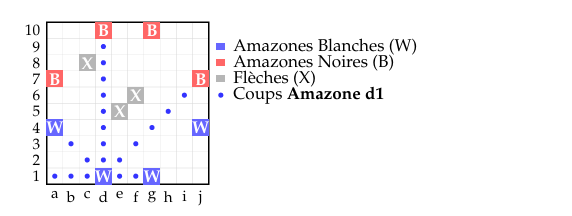
\includegraphics[width=0.58\textwidth]{schema_plateau.png}%
}{%
    \fbox{%
      \parbox[c][0.26\textheight][c]{0.75\linewidth}{%
        \centering Ajouter l'image \texttt{schema\_plateau.png}\\[0.5em]
        dans \texttt{pdp/02-final}
      }%
    }%
}
\caption{Vue synthétique du plateau avec coordonnées algébriques, amazones blanches et noires, flèches bloquantes et coups légaux illustrés pour l'amazone blanche sélectionnée.}
\label{fig:plateau_jeu}
\end{figure}

La Figure~\ref{fig:plateau_jeu} sert de référence visuelle pour la suite. Elle montre les coordonnées du plateau, la distinction entre amazones blanches (\texttt{W}), amazones noires (\texttt{B}) et flèches (\texttt{X}), ainsi qu'un exemple de coups légaux déjà calculés pour une amazone donnée. Les coordonnées utilisées dans les exemples textuels doivent être lues sur ce même repère.

\subsection{Placement adaptatif selon la taille du plateau}

La taille du plateau étant paramétrable, un placement unique des amazones n'aurait pas été satisfaisant. Le projet retient donc une stratégie adaptative dont l'objectif est de préserver une symétrie minimale et une jouabilité acceptable sur plusieurs dimensions :

\begin{table}[H]
\centering
\begin{tabular}{ccl}
\toprule
\textbf{Taille ($N \times N$)} & \textbf{Nb Amazones} & \textbf{Stratégie} \\
\midrule
$4 \times 4$ & 2 & Coins opposés \\
$5 \times 5$ & 3 & Triangle symétrique \\
$6 \times 6$ à $11 \times 11$ & 4 & Formule des Tiers \\
\bottomrule
\end{tabular}
\caption{Stratégies de placement selon la taille du plateau}
\end{table}

Pour $N \geq 6$, les positions sont calculées par l'algorithme des Tiers : $T = \lfloor N/3 \rfloor$, avec les amazones blanches placées aux positions $(0, T)$, $(0, N{-}1{-}T)$, $(T, 0)$ et $(T, N{-}1)$, et les noires par symétrie centrale. Ce choix maintient une distribution équilibrée sur les bords sans figer le moteur sur la seule configuration classique $10 \times 10$.

\subsection{Notation algébrique (F20)}

Les cases sont identifiées par une colonne (lettre \texttt{a} à \texttt{j}) et une ligne (chiffre \texttt{1} à \texttt{10}). Les coups suivent la notation algébrique standard :

\begin{center}
    \texttt{e2-e4/e6} $\rightarrow$ déplacer l'amazone de \texttt{e2} vers \texttt{e4}, puis tirer une flèche sur \texttt{e6}.
\end{center}

\begin{figure}[H]
\centering
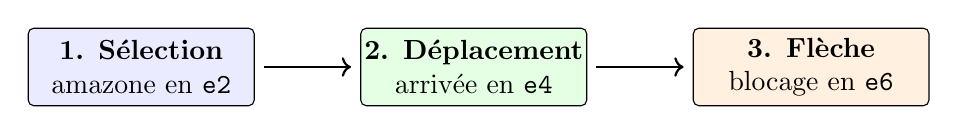
\begin{tikzpicture}[scale=0.82]
    \draw[rounded corners=2pt, fill=blue!8] (0,0) rectangle (3.5,1.2);
    \node[align=center] at (1.75,0.6) {\textbf{1. Sélection}\\amazone en \texttt{e2}};

    \draw[->, thick] (3.65,0.6) -- (5.0,0.6);

    \draw[rounded corners=2pt, fill=green!10] (5.15,0) rectangle (8.65,1.2);
    \node[align=center] at (6.9,0.6) {\textbf{2. Déplacement}\\arrivée en \texttt{e4}};

    \draw[->, thick] (8.8,0.6) -- (10.15,0.6);

    \draw[rounded corners=2pt, fill=orange!12] (10.3,0) rectangle (13.95,1.2);
    \node[align=center] at (12.125,0.6) {\textbf{3. Flèche}\\blocage en \texttt{e6}};
\end{tikzpicture}
\caption{Exemple concret d'un coup complet : \texttt{e2-e4/e6}.}
\label{fig:move-example}
\end{figure}

Cette notation sera réutilisée dans l'ensemble du projet. Dans le rapport, elle relie directement la description du coup, la Figure~\ref{fig:plateau_jeu} et l'exemple de la Figure~\ref{fig:move-example}.

%==============================================================================
%   SECTION 5 : CONCEPTION DU SYSTÈME
%==============================================================================

\section{Structures de données}

Cette section présente la représentation interne retenue pour manipuler le plateau. Le choix central est celui des bitboards : il répond au coût élevé des tests d'occupation, des mises à jour locales et de la génération répétée de coups.

\subsection{Bitboards}

Conformément aux exigences F26 et F27, le plateau est représenté par des \textbf{bitboards} \cite{browne2014}. Un bitboard est un entier de $n^2$ bits où chaque bit correspond à une case du plateau. L'état du jeu est encodé par \textbf{trois bitboards distincts} :

\begin{table}[H]
\centering
\begin{tabular}{lp{9cm}}
\toprule
\textbf{Bitboard} & \textbf{Contenu} \\
\midrule
\texttt{white\_bb} & Positions des amazones blanches \\
\texttt{black\_bb} & Positions des amazones noires \\
\texttt{arrow\_bb} & Positions des flèches (cases bloquées) \\
\bottomrule
\end{tabular}
\caption{Les trois bitboards représentant l'état du jeu}
\end{table}

Une matrice $N \times N$ aurait été plus intuitive, mais elle n'était pas la plus adaptée ici. Les bitboards ont été retenus pour trois raisons :
\begin{itemize}
    \item ils concentrent l'état du plateau dans quelques entiers ;
    \item ils rendent les tests d'occupation et les mises à jour très peu coûteux ;
    \item ils s'intègrent directement aux besoins du moteur et des IA, qui manipulent un grand nombre d'états successifs sans conversion intermédiaire vers une matrice ou une structure de graphe.
\end{itemize}

Le coût du choix est connu : l'indexation devient plus abstraite et le code moins immédiat à lire qu'avec une matrice. Ce compromis a été accepté parce que, dans ce projet, les opérations critiques ne lisent presque jamais le plateau pour l'afficher ; elles testent surtout des occupations, construisent des états temporaires et reviennent en arrière très souvent.

\subsubsection{Indexation des cases}

Chaque case possède un index unique : $\texttt{index} = \texttt{ligne} \times n + \texttt{colonne}$, avec ligne et colonne $\in [0, n{-}1]$.

\begin{table}[H]
\centering
\begin{tabular}{cccc}
\toprule
\textbf{Case (affichée)} & \textbf{Coord. interne} & \textbf{Calcul ($n=10$)} & \textbf{Index} \\
\midrule
\texttt{a1} & $(9, 0)$ & $9 \times 10 + 0$ & \textbf{90} \\
\texttt{d4} & $(6, 3)$ & $6 \times 10 + 3$ & \textbf{63} \\
\texttt{j10} & $(0, 9)$ & $0 \times 10 + 9$ & \textbf{9} \\
\bottomrule
\end{tabular}
\caption{Correspondance notation algébrique $\leftrightarrow$ index bitboard (plateau $10 \times 10$)}
\end{table}

\textit{Note :} l'indexation interne commence en haut à gauche, alors que la notation algébrique place \texttt{a1} en bas à gauche. La conversion \texttt{algèbre} $\rightarrow$ \texttt{index} doit donc inverser l'axe vertical, ce qui explique que \texttt{a1} ne corresponde pas à l'index 0 dans l'implémentation réelle.

\subsubsection{Opérations bit à bit}

Les opérations fondamentales permettent de manipuler l'état du plateau en temps constant $O(1)$ :

\begin{table}[H]
\centering
\begin{tabular}{lll}
\toprule
\textbf{Opération} & \textbf{Notation} & \textbf{Usage} \\
\midrule
Shift gauche & $1 \ll n$ & Créer un masque pour la position $n$ \\
OR & $a \mid b$ & Placer une pièce ou bloquer une case \\
XOR & $a \oplus b$ & Retirer une pièce (inverser un bit) \\
AND & $a \land b$ & Tester si une case est occupée \\
\bottomrule
\end{tabular}
\caption{Récapitulatif des opérations bit à bit}
\end{table}

\textbf{Application d'un coup} (ordre strict) :
\begin{enumerate}
    \item \textbf{Libérer} la case de départ : $\texttt{amazons} = \texttt{amazons} \oplus (1 \ll \texttt{from})$
    \item \textbf{Occuper} la case d'arrivée : $\texttt{amazons} = \texttt{amazons} \mid (1 \ll \texttt{to})$
    \item \textbf{Tirer la flèche} : $\texttt{arrows} = \texttt{arrows} \mid (1 \ll \texttt{arrow})$
\end{enumerate}

\textit{Note :} L'ordre est crucial car la flèche peut légalement atterrir sur la case \texttt{from} libérée à l'étape 1.

\subsubsection{Visualisation des opérations critiques}

Les figures suivantes détaillent deux opérations centrales du moteur bitboard : la détection d'une collision sur un chemin de déplacement, puis l'écriture effective d'un déplacement dans les structures binaires.

\paragraph{Validation d'un coup (lecture)}

Pour vérifier si un coup est valide, le moteur agrège d'abord les obstacles (\texttt{OR}), construit ensuite un masque correspondant au chemin voulu, puis teste l'intersection via \texttt{AND}. Toute intersection non nulle signale une collision.

\begin{figure}[H]
\centering
\begin{minipage}{0.31\textwidth}
\centering
\textbf{1. Occupation (OR)}\\[0.3em]
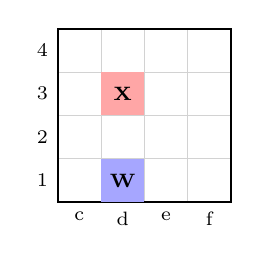
\begin{tikzpicture}[scale=0.55]
    \draw[step=1cm, gray!35, very thin] (0,0) grid (4,4);
    \draw[thick] (0,0) rectangle (4,4);
    \foreach \x/\l in {0/c,1/d,2/e,3/f} {
        \node[below, font=\scriptsize] at (\x+0.5,0) {\l};
    }
    \foreach \y/\l in {0/1,1/2,2/3,3/4} {
        \node[left, font=\scriptsize] at (0,\y+0.5) {\l};
    }
    \fill[blue!35] (1,0) rectangle (2,1);
    \fill[red!35] (1,2) rectangle (2,3);
    \node[font=\scriptsize\bfseries] at (1.5,0.5) {W};
    \node[font=\scriptsize\bfseries] at (1.5,2.5) {X};
\end{tikzpicture}
\end{minipage}\hfill
\begin{minipage}{0.31\textwidth}
\centering
\textbf{2. Masque du trajet}\\[0.3em]
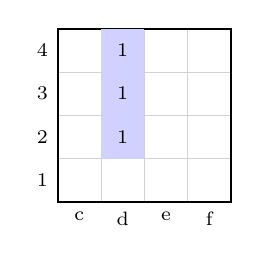
\begin{tikzpicture}[scale=0.55]
    \draw[step=1cm, gray!35, very thin] (0,0) grid (4,4);
    \draw[thick] (0,0) rectangle (4,4);
    \foreach \x/\l in {0/c,1/d,2/e,3/f} {
        \node[below, font=\scriptsize] at (\x+0.5,0) {\l};
    }
    \foreach \y/\l in {0/1,1/2,2/3,3/4} {
        \node[left, font=\scriptsize] at (0,\y+0.5) {\l};
    }
    \fill[blue!18] (1,1) rectangle (2,2);
    \fill[blue!18] (1,2) rectangle (2,3);
    \fill[blue!18] (1,3) rectangle (2,4);
    \node[font=\scriptsize] at (1.5,1.5) {1};
    \node[font=\scriptsize] at (1.5,2.5) {1};
    \node[font=\scriptsize] at (1.5,3.5) {1};
\end{tikzpicture}
\end{minipage}\hfill
\begin{minipage}{0.31\textwidth}
\centering
\textbf{3. Collision (AND)}\\[0.3em]
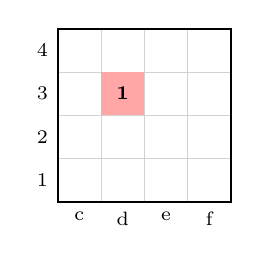
\begin{tikzpicture}[scale=0.55]
    \draw[step=1cm, gray!35, very thin] (0,0) grid (4,4);
    \draw[thick] (0,0) rectangle (4,4);
    \foreach \x/\l in {0/c,1/d,2/e,3/f} {
        \node[below, font=\scriptsize] at (\x+0.5,0) {\l};
    }
    \foreach \y/\l in {0/1,1/2,2/3,3/4} {
        \node[left, font=\scriptsize] at (0,\y+0.5) {\l};
    }
    \fill[red!35] (1,2) rectangle (2,3);
    \node[font=\scriptsize\bfseries] at (1.5,2.5) {1};
\end{tikzpicture}
\end{minipage}

\vspace{0.5em}

{\small Le masque de déplacement sur la colonne \texttt{d} rencontre une case déjà occupée en \texttt{d3} ; l'intersection est donc non nulle et le coup est refusé.}
\caption{Validation d'un coup : l'opération \texttt{AND} détecte la collision sur un plateau $10 \times 10$.}
\label{fig:bitboard_collision}
\end{figure}

La validité d'un déplacement est donc ramenée à une suite d'opérations binaires sur des masques de trajet et d'occupation, et non à un parcours matriciel case par case.

\paragraph{Application d'un coup (écriture)}

Le déplacement ne se fait pas par copie de plateau, mais par modification ciblée de bits : on retire d'abord l'amazone de sa case de départ par \texttt{XOR}, puis on active la case d'arrivée par \texttt{OR}.

\begin{figure}[H]
\centering
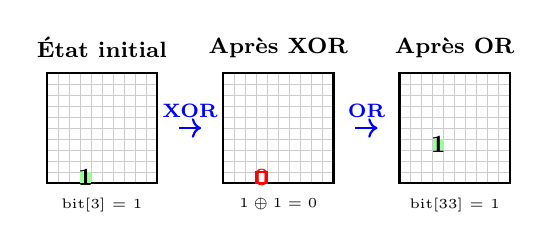
\begin{tikzpicture}[scale=0.14]
    \tikzset{
        gridstyle/.style={step=1cm, gray!40, very thin},
        borderstyle/.style={thick, black}
    }

    \begin{scope}
        \draw[gridstyle] (0,0) grid (10,10);
        \draw[borderstyle] (0,0) rectangle (10,10);
        \node[above] at (5,10.5) {\footnotesize \textbf{État initial}};
        \fill[green!40] (3,0) rectangle (4,1);
        \node[font=\small\bfseries] at (3.5,0.5) {1};
        \node[below] at (5,-0.5) {\tiny bit[3] = 1};
    \end{scope}

    \draw[->, thick, blue] (12,5) -- (14,5)
        node[midway, above, font=\scriptsize] {\textbf{XOR}};

    \begin{scope}[xshift=16cm]
        \draw[gridstyle] (0,0) grid (10,10);
        \draw[borderstyle] (0,0) rectangle (10,10);
        \node[above] at (5,10.5) {\footnotesize \textbf{Après XOR}};
        \draw[red, thick] (3,0) rectangle (4,1);
        \node[red, font=\small\bfseries] at (3.5,0.5) {0};
        \node[below] at (5,-0.5) {\tiny $1 \oplus 1 = 0$};
    \end{scope}

    \draw[->, thick, blue] (28,5) -- (30,5)
        node[midway, above, font=\scriptsize] {\textbf{OR}};

    \begin{scope}[xshift=32cm]
        \draw[gridstyle] (0,0) grid (10,10);
        \draw[borderstyle] (0,0) rectangle (10,10);
        \node[above] at (5,10.5) {\footnotesize \textbf{Après OR}};
        \fill[green!40] (3,3) rectangle (4,4);
        \node[font=\small\bfseries] at (3.5,3.5) {1};
        \node[below] at (5,-0.5) {\tiny bit[33] = 1};
    \end{scope}

\end{tikzpicture}
\caption{Déplacement d'une amazone : \texttt{XOR} retire, \texttt{OR} place (plateau $10 \times 10$).}
\label{fig:bitboard_move}
\end{figure}

Cette représentation montre l'intérêt pratique des bitboards : un déplacement complet se traduit par quelques opérations élémentaires sur des entiers, sans recopier tout le plateau. Cet avantage devient déterminant lorsqu'une IA doit tester un grand nombre de coups successifs.

\section{Algorithmes}

Cette section présente d'abord la génération et la validation des coups, puis les moteurs d'intelligence artificielle. L'objectif est de montrer comment le système passe d'un état de jeu encodé à une décision exploitable.

\subsection{Génération et validation des coups}

La génération des coups légaux constitue l'opération la plus critique du moteur. Dans le code, elle apparaît comme un générateur : l'entrée est la couleur à jouer et l'occupation courante du plateau ; la sortie est un flux de triplets \texttt{Move(from, to, arrow)} produits un par un. Pour chaque amazone, on explore les 8 directions cardinales et diagonales :
\[
DIRS = \{(+1,0), (-1,0), (0,+1), (0,-1), (+1,+1), (-1,-1), (+1,-1), (-1,+1)\}
\]

Conceptuellement, ces directions se traduisent sur le bitboard 1D par des décalages d'index. Dans l'implémentation réelle, le moteur procède toutefois plus prudemment : il reconstruit d'abord la ligne et la colonne de la case courante, applique un couple $(\Delta ligne,\Delta colonne)$, puis reconvertit en index seulement après validation des bornes. Cette étape évite de fabriquer des indices valides en apparence mais faux géométriquement.

Sur un plateau de largeur $L = n$, les directions correspondent ainsi aux variations suivantes :
\begin{itemize}
    \item \textbf{Vertical} : Nord ($+n$), Sud ($-n$)
    \item \textbf{Horizontal} : Est ($+1$), Ouest ($-1$)
    \item \textbf{Diagonal} : NE ($+n{+}1$), NO ($+n{-}1$), SE ($-n{+}1$), SO ($-n{-}1$)
\end{itemize}

\subsubsection{Problème du wrapping}

L'indexation linéaire crée une fausse continuité entre les bords du plateau. Par exemple, l'index $9$ (colonne $j$, ligne $1$) $+ 1$ donne l'index $10$ (colonne $a$, ligne $2$) : une téléportation indésirable.

\textbf{Solution retenue dans le code :}
\begin{itemize}
    \item convertir l'index courant en coordonnées \texttt{(row, col)} ;
    \item avancer par \texttt{row += dr} et \texttt{col += dc} ;
    \item interrompre la propagation dès que \texttt{row} ou \texttt{col} sort de $[0, n{-}1]$ ;
    \item ne reconstruire l'index \texttt{row * size + col} qu'après ce contrôle.
\end{itemize}

Cette solution est légèrement moins ``bit trick'' qu'un système de masques de bords, mais elle est plus lisible et colle exactement à la géométrie du jeu. Elle supprime le wrapping pour les mouvements horizontaux comme pour les diagonales avec une seule règle de borne.

\subsubsection{Algorithme complet}

Pour chaque amazone à la position $P$ et chaque direction $D$ :
\begin{enumerate}
    \item Initialiser $cur = P$.
    \item Convertir $cur$ en coordonnées $(row, col)$ puis calculer $(row + dr, col + dc)$.
    \item \textbf{Bornes / anti-wrap} : si l'une des deux coordonnées sort du plateau, arrêter.
    \item Reconstruire $next = row \times n + col$.
    \item \textbf{Collision} : si $next$ est occupé (test bit à 1 dans \texttt{occupied}), arrêter.
    \item Ajouter $next$ aux destinations valides, avancer ($cur = next$), retour à l'étape 2.
    \item Pour chaque destination $to$, recalculer une occupation temporaire où la case de départ est libérée et la case d'arrivée devient occupée.
    \item Relancer exactement le même itérateur depuis $to$ pour générer les positions de flèche.
\end{enumerate}

La procédure reste simple, mais elle est appelée partout : moteur, évaluateurs et algorithmes de recherche. Le déroulement complet du coup \texttt{e2-e4/e6} est détaillé plus loin dans la Section~\ref{sec:explication-approfondie}.

\begin{figure}[H]
  \centering
  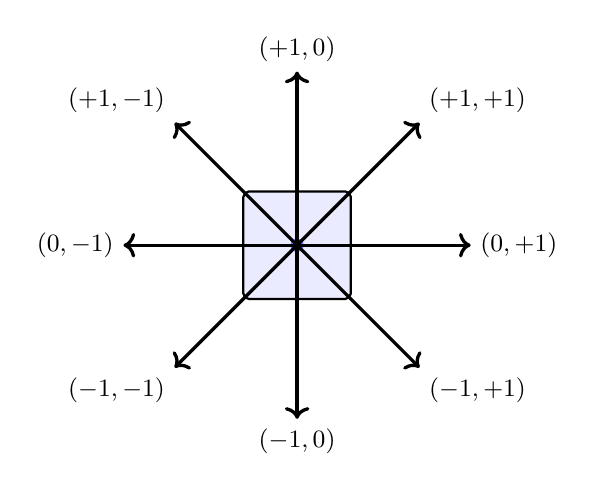
\begin{tikzpicture}[scale=1.05]
    \draw[rounded corners=2pt, thick, fill=blue!8] (-0.65,-0.65) rectangle (0.65,0.65);
    \draw[blue!50, thick] (-0.65,0) -- (0.65,0);
    \draw[blue!50, thick] (0,-0.65) -- (0,0.65);
    \draw[blue!50, thick] (-0.46,-0.46) -- (0.46,0.46);
    \draw[blue!50, thick] (-0.46,0.46) -- (0.46,-0.46);
    \fill[blue!55] (0,0) circle (0.08);

    \draw[->, very thick] (0,0) -- (0,2.1);
    \draw[->, very thick] (0,0) -- (1.48,1.48);
    \draw[->, very thick] (0,0) -- (2.1,0);
    \draw[->, very thick] (0,0) -- (1.48,-1.48);
    \draw[->, very thick] (0,0) -- (0,-2.1);
    \draw[->, very thick] (0,0) -- (-1.48,-1.48);
    \draw[->, very thick] (0,0) -- (-2.1,0);
    \draw[->, very thick] (0,0) -- (-1.48,1.48);

    \node[above, font=\small] at (0,2.1) {$(+1,0)$};
    \node[above right, font=\small] at (1.48,1.48) {$(+1,+1)$};
    \node[right, font=\small] at (2.1,0) {$(0,+1)$};
    \node[below right, font=\small] at (1.48,-1.48) {$(-1,+1)$};
    \node[below, font=\small] at (0,-2.1) {$(-1,0)$};
    \node[below left, font=\small] at (-1.48,-1.48) {$(-1,-1)$};
    \node[left, font=\small] at (-2.1,0) {$(0,-1)$};
    \node[above left, font=\small] at (-1.48,1.48) {$(+1,-1)$};
  \end{tikzpicture}
  \caption[Huit directions de propagation autour d'une amazone.]{Huit directions de propagation autour d'une amazone, exprimées en déplacements $(\Delta ligne,\Delta colonne)$.}
  \label{fig:algo-propagation}
\end{figure}

Cette synthèse aide à comprendre que la génération d'un coup légal combine plusieurs contrôles successifs : les bords du plateau, l'absence de collision, puis la génération des cases de tir de flèche. Elle explicite donc la différence entre un simple déplacement et un coup complet des Amazones.

\subsection{Algorithmes d'intelligence artificielle}

\subsubsection{Minimax avec élagage \texorpdfstring{$\alpha\beta$}{alpha-beta}}

L'algorithme Minimax \cite{knuth1975} explore un arbre alternant des niveaux \textbf{MAX} et \textbf{MIN}. Son intérêt principal, dans notre projet, est sa bonne intégration au moteur existant : le même \texttt{Board} fournit les coups légaux, applique un coup, annule ce coup et expose l'état au scoreur. Sa limite est immédiate sur les Amazones : avec un facteur de branchement $b$ élevé, le coût d'une recherche de profondeur $d$ reste de l'ordre de $O(b^d)$ et croît très vite.

L'élagage $\alpha\beta$ réduit considérablement le nombre de nœuds explorés en coupant les branches dont on sait qu'elles ne peuvent pas influencer la décision finale :
\[
\text{Coupure si } \alpha \geq \beta
\]

Cette optimisation ne change pas la nature exponentielle du problème, mais elle améliore nettement le comportement pratique. Dans le projet, Minimax reste utile pour obtenir un comportement déterministe, traçable et stable sur des profondeurs modestes. La recherche est bornée par une profondeur configurable et par un budget temps, puis les feuilles sont évaluées par des heuristiques.

Techniquement, la méthode \texttt{best\_move} construit d'abord la liste des coups légaux, applique chaque coup candidat, appelle \texttt{minimax(...)} puis restaure exactement le plateau. La récursion s'arrête en cas de profondeur nulle, d'absence de coups légaux ou de dépassement du budget temps. Le détail pas à pas et les tests associés sont donnés dans la Section~\ref{sec:explication-approfondie}.

\subsubsection{Fonctions d'évaluation}

Trois heuristiques sont implémentées. Elles correspondent à trois lectures différentes d'une bonne position :

\textbf{Mobilité} \cite{muller2002} :
\[
score_{mob}(s) = |Moves(s, joueur)| - |Moves(s, adversaire)|
\]

\textbf{Territoire} \cite{lieberum1999} (propagation locale depuis l'ensemble des amazones d'un camp) :
\[
score_{terr}(s) = \#cases_{nous} - \#cases_{adversaire}
\]

\textbf{Hybride} (combinaison pondérée) :
\[
score_{hyb}(s) = 0.6 \cdot score_{terr}(s) + 0.4 \cdot score_{mob}(s)
\]

Dans l'implémentation actuelle, l'évaluateur de territoire ne calcule pas une compétition de distances minimales case par case. Il effectue un \emph{flood-fill} en voisinage de roi depuis toutes les amazones d'un camp, puis compte les cases atteignables. L'heuristique reste donc spatiale, mais volontairement simple et rapide.

L'évaluateur hybride combine mobilité et territoire pour mieux couvrir les différentes phases de la partie. Le code retient un compromis fixe $0.6/0.4$ : la pondération est stable et simple à utiliser, mais elle n'est pas encore ajustée dynamiquement selon la position.

\subsubsection{Monte Carlo Tree Search (MCTS)}

MCTS \cite{browne2012mcts} explore l'arbre de jeu par simulations successives. Cette approche est intéressante pour les Amazones car elle supporte mieux les très grands facteurs de branchement qu'une recherche Minimax profonde. Au lieu de fixer d'emblée une profondeur, MCTS investit progressivement le budget temps dans les branches les plus prometteuses :

\begin{enumerate}
    \item \textbf{Sélection} : descendre dans l'arbre en choisissant les nœuds selon une variante du critère UCT \cite{kocsis2006uct}. Dans notre code, chaque nœud stocke ses victoires du point de vue du joueur qui doit jouer à ce nœud. La sélection inverse donc le taux de victoire de l'enfant pour raisonner du point de vue du parent, puis ajoute un terme d'exploration.
    \item \textbf{Expansion} : ajouter un nœud fils non exploré.
    \item \textbf{Simulation} (rollout) : jouer aléatoirement jusqu'à la fin de partie.
    \item \textbf{Rétropropagation} : mettre à jour les statistiques ($w_i$, $n_i$) de chaque nœud traversé.
\end{enumerate}

L'avantage principal de cette approche est sa nature \emph{anytime} : plus on lui accorde de temps, plus les statistiques se raffinent, sans profondeur fixe imposée à l'avance. En contrepartie, la qualité du résultat dépend fortement de la politique de simulation et du réglage exploration/exploitation. Dans notre implémentation, les rollouts restent simples ; cela préserve la lisibilité du code, mais limite la qualité stratégique des estimations.

\subsubsection{Comparaison critique des approches}

Minimax et MCTS ne répondent pas au même besoin. Minimax convient mieux quand on veut une décision stable et justifiable par une heuristique explicite. MCTS supporte mieux les grands facteurs de branchement et utilise le temps disponible de façon plus souple, au prix d'une décision moins lisible. Garder les deux moteurs permet donc de comparer deux stratégies de décision sous contrainte de temps.

%==============================================================================
%   SECTION 3 : ARCHITECTURE DU PROJET
%==============================================================================

\section{Architecture du système}

L'architecture du système repose sur une idée simple : un même noyau métier doit servir tous les modes d'utilisation. La CLI, la GUI, l'IA, la sauvegarde et le réseau ne redéfinissent pas les règles ; ils réutilisent les mêmes opérations de validation et les mêmes structures de données.

La Figure~\ref{fig:global-workflow} ne représente pas une hiérarchie de classes. Elle résume le chemin fonctionnel principal d'une action utilisateur dans le système.

\begin{figure}[H]
\centering
{\small\itshape
Vue (CLI / GUI) $\rightarrow$ GameController $\rightarrow$ Board $\rightarrow$ Player $\rightarrow$ Move\par
}
\caption{Workflow global du système : de l'action utilisateur jusqu'au coup validé.}
\label{fig:global-workflow}
\end{figure}

Ce schéma résume le flux principal du projet. La vue transmet une intention d'action au contrôleur, le contrôleur s'appuie sur \texttt{Board} pour valider l'état et délègue ensuite l'obtention du coup au joueur courant, qu'il soit humain, IA ou réseau. Le résultat reste un objet \texttt{Move} unique, ce qui garantit un traitement homogène entre tous les modes de jeu.

Le rôle de la vue doit être précisé. \texttt{ViewCli} lit des commandes textuelles, affiche l'état de la partie et relaie les demandes utilisateur. \texttt{ViewGui} capte des événements GTK, dessine le plateau et orchestre les interactions visuelles. Aucune de ces vues ne décide elle-même si un coup est légal. Elles collectent des intentions d'action, puis les transmettent à \texttt{GameController}. Cette séparation est essentielle : elle évite d'avoir une règle implémentée une fois en CLI et une autre en GUI.

Dans l'implémentation actuelle, cette chaîne reste pilotée par \texttt{GameController}, mais une partie du traitement passe désormais par les modules auxiliaires de \texttt{controller/engine}. Le pipeline reste donc volontairement simple dans le rapport, tout en correspondant à une implémentation devenue plus modulaire.

La Figure~\ref{fig:ai-pipeline} joue le même rôle pour la décision artificielle : elle présente un enchaînement fonctionnel, pas une liste de classes.

\begin{figure}[H]
\centering
{\small\itshape
Board $\rightarrow$ legal moves $\rightarrow$ search engine $\rightarrow$ best move\par
}
\caption{Pipeline de décision de l'intelligence artificielle.}
\label{fig:ai-pipeline}
\end{figure}

Le pipeline IA clarifie le rôle des différents composants. Le plateau fournit l'état courant et les coups légaux. Un moteur de recherche exploite ensuite cet espace de décision. Selon le moteur choisi, la décision repose soit sur une évaluation heuristique, soit sur des simulations. Le résultat final reste un coup concret, directement exploitable par le contrôleur.

\subsection{Architecture générale}

\subsubsection{Pattern MVC}

L'architecture suit le patron \textbf{Modèle-Vue-Contrôleur} (MVC) \cite{gamma1994}, avec l'objectif de séparer la logique métier, les mécanismes d'orchestration et les interfaces utilisateur :

\begin{table}[H]
\centering
\begin{tabular}{lll}
\toprule
\textbf{Couche} & \textbf{Responsabilité} & \textbf{Répertoires principaux} \\
\midrule
\textbf{Model} & Données et logique métier & \texttt{model/} \\
\textbf{View} & Affichage et interaction utilisateur & \texttt{view/ui/} \\
\textbf{Controller} & Orchestration et flux de jeu & \texttt{controller/}, \texttt{controller/engine/}, \texttt{controller/network/} \\
\bottomrule
\end{tabular}
\caption{Découpage MVC du projet}
\end{table}

Dans notre implémentation, le modèle encapsule les invariants du jeu et les structures de données partagées ; la vue se limite, dans l'intention, à la présentation et à la collecte des interactions ; le contrôleur convertit enfin ces interactions en opérations métier. Ce découpage a été retenu pour une raison concrète : les mêmes règles doivent être appelées depuis la CLI, la GUI, l'IA et le réseau. Sans cette séparation, la validation des coups et la gestion de l'état auraient été dupliquées dans plusieurs interfaces.

Dans les faits, le contrôleur centralise toutefois une part importante des dépendances entre couches. Il instancie le plateau, les joueurs humains, IA ou réseau, délègue l'affichage à la CLI ou à la GUI, et coordonne la sauvegarde, le chargement, l'historique, le chronométrage et les échanges réseau. Ce choix a simplifié l'intégration initiale du projet, mais il a un coût clair : \texttt{GameController} reste le point où se concentrent plusieurs causes de changement. Le code actuel a commencé à extraire certaines responsabilités vers des modules spécialisés de \texttt{controller/engine}, ce qui améliore la lisibilité sans supprimer encore cette centralisation.

L'architecture générale reste simple. Le noyau métier repose sur \texttt{Board}, \texttt{Move}, la hiérarchie des joueurs et les moteurs d'IA. La persistance, le réseau et l'internationalisation jouent un rôle transverse. La CLI et la GUI sont deux entrées vers ce même noyau. Dans le code actuel, la couche contrôleur ne se limite plus à \texttt{game\_controller.py} : une partie de la logique a été déplacée dans \texttt{controller/engine}. \texttt{GameController} reste toutefois la façade centrale. Cette factorisation améliore la lecture locale, mais le couplage reste fort.

\subsubsection{Découpage en modules}

\begin{figure}[H]
  \centering
  \resizebox{0.98\textwidth}{!}{%
  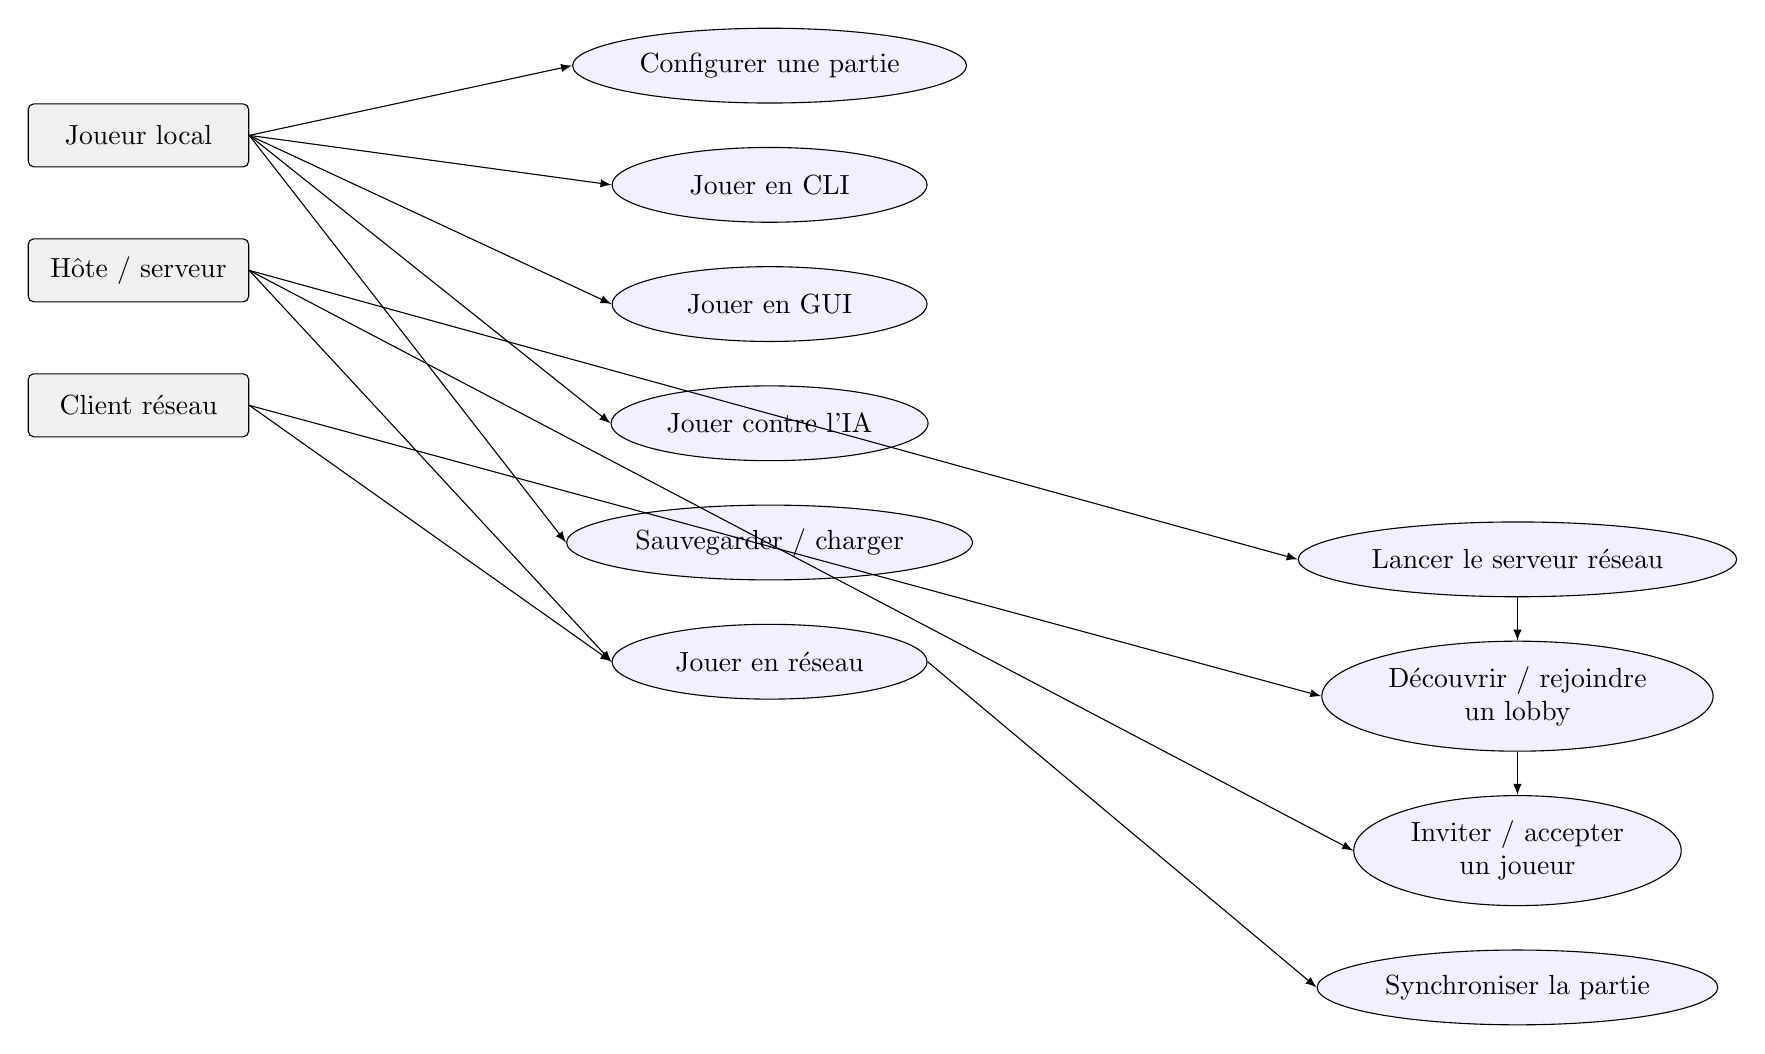
\begin{tikzpicture}[
    actor/.style={draw, rounded corners=2pt, fill=gray!12, minimum width=2.8cm, minimum height=0.8cm, align=center},
    usecase/.style={draw, ellipse, fill=blue!6, minimum width=4.0cm, minimum height=0.95cm, align=center},
    node distance=1.0cm and 2.4cm,
  ]
    \node[actor] (local) {Joueur local};
    \node[actor, below=0.9cm of local] (host) {Hôte / serveur};
    \node[actor, below=0.9cm of host] (client) {Client réseau};

    \node[usecase, right=4.1cm of host, yshift=2.6cm] (config) {Configurer une partie};
    \node[usecase, below=0.55cm of config] (cli) {Jouer en CLI};
    \node[usecase, below=0.55cm of cli] (gui) {Jouer en GUI};
    \node[usecase, below=0.55cm of gui] (ai) {Jouer contre l'IA};
    \node[usecase, below=0.55cm of ai] (save) {Sauvegarder / charger};
    \node[usecase, below=0.55cm of save] (network) {Jouer en réseau};
    \node[usecase, right=4.7cm of network, yshift=1.3cm] (server) {Lancer le serveur réseau};
    \node[usecase, below=0.55cm of server] (lobby) {Découvrir / rejoindre\\un lobby};
    \node[usecase, below=0.55cm of lobby] (invite) {Inviter / accepter\\un joueur};
    \node[usecase, below=0.55cm of invite] (sync) {Synchroniser la partie};

    \draw[-latex] (local.east) -- (config.west);
    \draw[-latex] (local.east) -- (cli.west);
    \draw[-latex] (local.east) -- (gui.west);
    \draw[-latex] (local.east) -- (ai.west);
    \draw[-latex] (local.east) -- (save.west);

    \draw[-latex] (host.east) -- (server.west);
    \draw[-latex] (host.east) -- (invite.west);
    \draw[-latex] (host.east) -- (network.west);

    \draw[-latex] (client.east) -- (lobby.west);
    \draw[-latex] (client.east) -- (network.west);

    \draw[-latex] (server.south) -- (lobby.north);
    \draw[-latex] (lobby.south) -- (invite.north);
    \draw[-latex] (network.east) -- (sync.west);
  \end{tikzpicture}
  }
  \caption{Diagramme de cas d'utilisation des fonctionnalités principales, incluant explicitement le serveur réseau et le lobby.}
  \label{fig:use-cases}
\end{figure}

Le diagramme de cas d'utilisation montre que l'IA, le réseau, la sauvegarde et la GUI prolongent le scénario central de jeu au lieu de constituer des applications séparées. Il fait aussi apparaître explicitement la partie \emph{serveur réseau}, qui ne se limite pas au transport des coups : démarrage du serveur, gestion du lobby, invitations et synchronisation des sessions font partie intégrante du système.

\begin{figure}[H]
  \centering
  \IfFileExists{class1.png}{%
    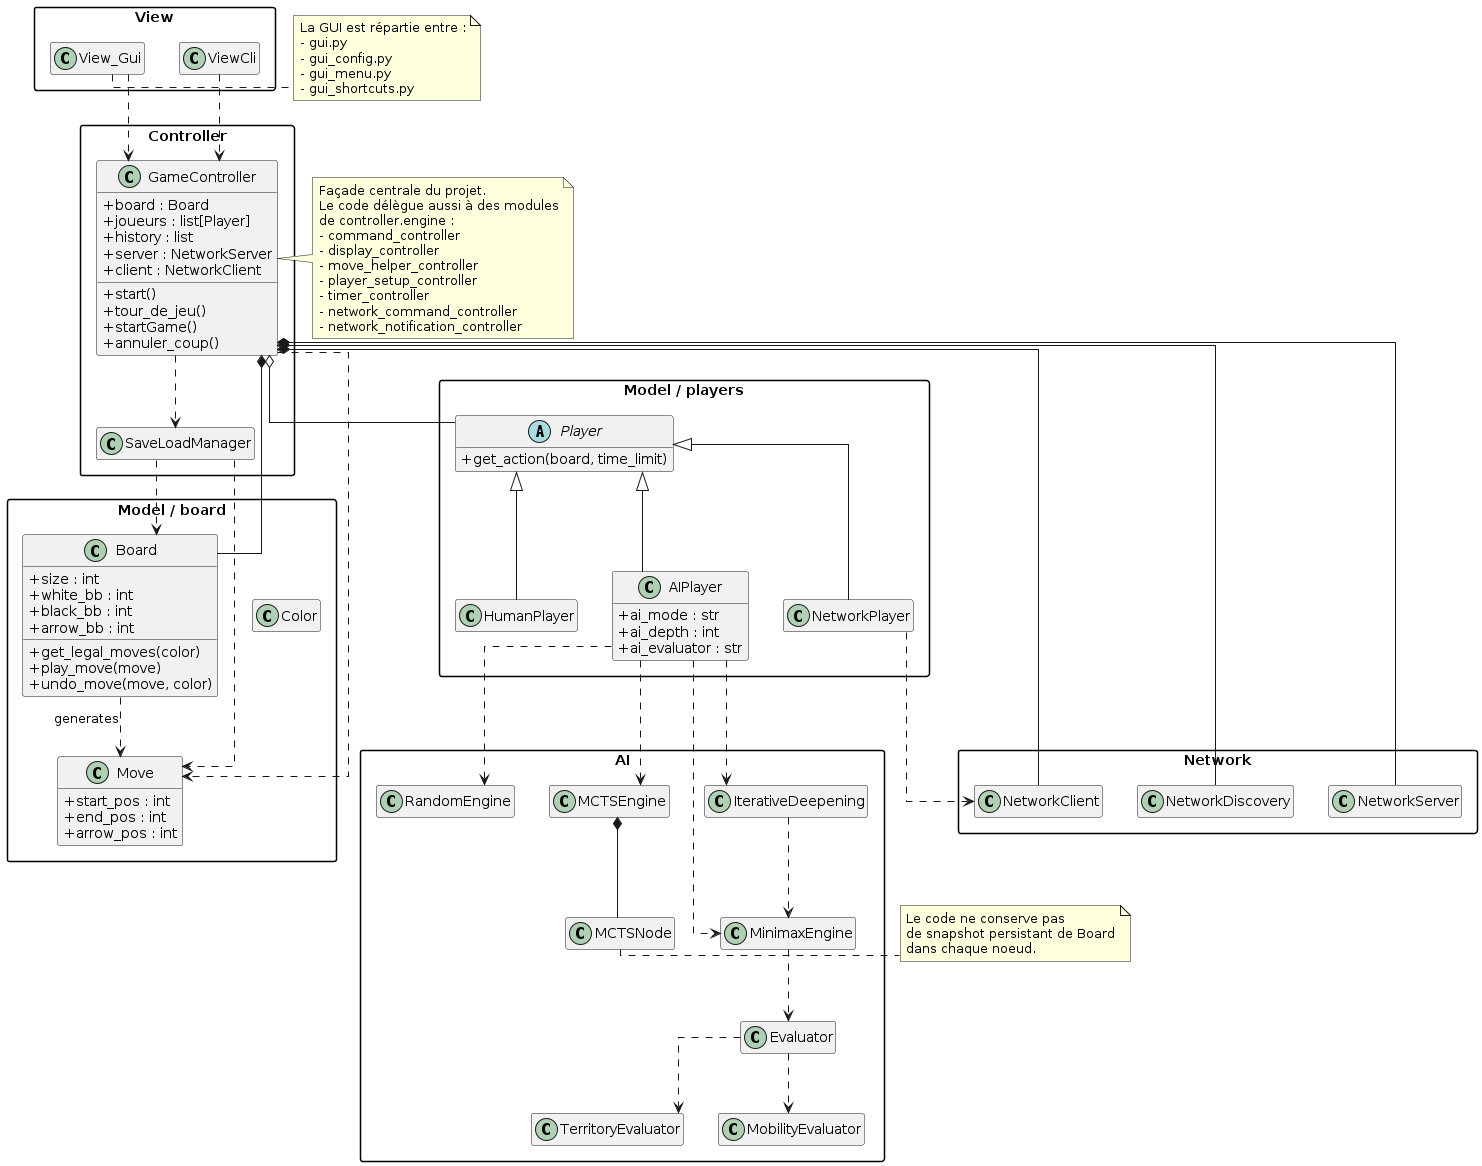
\includegraphics[width=0.95\textwidth]{class1.png}%
  }{%
    \IfFileExists{class1.pdf}{%
      \includegraphics[width=0.95\textwidth]{class1.pdf}%
    }{%
      \fbox{%
        \parbox[c][0.28\textheight][c]{0.75\linewidth}{%
          \centering Ajouter le diagramme de classes\\[0.4em]
          \texttt{class1.png} ou \texttt{class1.pdf}
        }%
      }%
    }%
  }
  \caption{Diagramme de classes UML du noyau structurant du projet.}\label{fig:classes}
\end{figure}

Le diagramme de classes a été volontairement limité aux classes réellement structurantes du projet. On y retrouve le noyau métier (\texttt{Board}, \texttt{Move}, \texttt{Player}), les spécialisations de joueurs, les moteurs d'IA, les vues CLI et GUI, ainsi que les services de persistance et de réseau manipulés par le contrôleur. Ce choix permet de garder une lecture claire du système sans mélanger structure objet et découpage modulaire.

La séparation récente de \texttt{controller/engine} n'apparaît donc pas sous la forme de nouvelles classes dans ce diagramme. C'est un point important : \texttt{command\_controller.py}, \texttt{display\_controller.py}, \texttt{timer\_controller.py} et les autres fichiers du dossier factorisent la logique du contrôleur, mais ils ne définissent pas pour autant des objets métier autonomes. Le diagramme de classes doit rester fidèle à la structure objet réelle ; la factorisation modulaire du contrôleur est, elle, expliquée dans le texte d'architecture.

\subsubsection{Module Model}

\begin{itemize}
    \item \path{board/board.py} : classe \texttt{Board} encapsulant les trois bitboards, la validation des coups et les transitions d'état principales du plateau.
    \item \path{board/move.py} : classe \texttt{Move} (triplet \texttt{start\_pos}, \texttt{end\_pos}, \texttt{arrow\_pos}) avec conversion algébrique $\leftrightarrow$ index.
    \item \path{players/} : hiérarchie de joueurs --- \texttt{HumanPlayer}, \texttt{AIPlayer}, \texttt{NetworkPlayer}.
    \item \path{ai/} : moteurs d'IA (\path{minimax_engine.py}, \path{iterative_deepening.py}, \path{mcts_engine.py}, \path{random_engine.py}) et évaluateurs (\path{mobility_evaluator.py}, \path{territory_evaluator.py}, combinaison hybride dans \path{evaluator.py}).
\end{itemize}

\subsubsection{Module Controller}

\begin{itemize}
    \item \path{engine/game_controller.py} : classe centrale \texttt{GameController}, responsable de la boucle de jeu et de l'orchestration applicative.
    \item Modules de commande et d'orchestration locale : \path{engine/command_controller.py}, \path{display_controller.py}, \path{move_helper_controller.py}, \path{player_setup_controller.py} et \path{timer_controller.py}.
    \item \path{engine/network_command_controller.py} et \path{network_notification_controller.py} : modules dédiés à une partie des échanges et notifications réseau, toujours branchés sur le même objet \texttt{GameController}.
    \item \path{save_load_manager.py} : service de sérialisation et de reconstruction des parties au format ASCII, avec contrôle de cohérence et checksum anti-triche.
    \item \path{network/} : services réseau TCP/UDP pour la découverte, la connexion, les invitations, la synchronisation des coups et la gestion des sessions distantes.
\end{itemize}

La factorisation engagée dans \texttt{controller/engine} améliore la lisibilité et limite la croissance du fichier principal. Elle ne constitue pas encore un vrai découplage : les modules auxiliaires restent branchés sur le même état contrôleur, et plusieurs responsabilités restent concentrées autour de \texttt{GameController}. Le projet est donc passé d'un contrôleur monolithique à une façade centrale entourée de modules spécialisés. Le gain est réel, mais incomplet.

\subsubsection{Module View}

\begin{itemize}
    \item \path{ui/cli.py} : interface en ligne de commande avec shell interactif, complétion, affichage du plateau, aide contextuelle et commandes réseau.
    \item \path{ui/gui.py}, \path{ui/gui_config.py}, \path{ui/gui_menu.py} et \path{ui/gui_shortcuts.py} : interface graphique GTK4, écran de configuration, affichage du plateau, menus, raccourcis clavier personnalisables, sauvegarde/chargement, interactions réseau et gestion du lobby graphique.
\end{itemize}

La coexistence de deux vues complètes n'est pas un simple confort d'utilisation. C'est un test architectural : si le moteur et le contrôleur sont correctement conçus, la même logique métier doit pouvoir être pilotée par une boucle CLI, par des callbacks GTK et par des événements réseau. Cette pluralité d'interfaces distingue le projet d'un prototype limité à un mode d'interaction unique.

\subsubsection{Interfaces principales entre modules}

Au-delà du découpage en dossiers, quelques interfaces structurent réellement le projet :

\begin{itemize}
    \item \textbf{Interface du plateau} : \texttt{Board} expose les opérations essentielles au reste du système, comme \texttt{get\_legal\_moves}, \texttt{is\_valid\_move}, \texttt{make\_move}, \texttt{undo\_move} et \texttt{get\_board\_array}. Cette API est utilisée à la fois par le contrôleur, les IA et la vue.
    \item \textbf{Interface de persistance} : \texttt{SaveLoadManager} joue le rôle de service transversal. Le contrôleur et la GUI s'appuient dessus pour sérialiser et reconstruire une partie sans dupliquer la logique.
    \item \textbf{Interface joueur} : la hiérarchie des joueurs permet au contrôleur de traiter de manière homogène un humain, une IA ou un joueur réseau, même si la récupération effective du coup diffère selon le type.
    \item \textbf{Interface vue} : la CLI et la GUI ne calculent pas les coups elles-mêmes ; elles transmettent des intentions d'action à la façade \texttt{GameController}, qui délègue ensuite une partie du traitement aux modules spécialisés de \texttt{controller/engine}.
\end{itemize}

Cette séparation reste partielle : \texttt{GameController} conserve encore beaucoup de responsabilités. Nous avons accepté ce compromis pour intégrer rapidement les sous-modules pendant le développement. La dette principale est claire : une future version devrait extraire la gestion des tours, le réseau, la persistance et l'orchestration GUI/CLI dans des services distincts.

\subsubsection{Diagrammes de séquence}

\begin{figure}[H]
  \centering
  \IfFileExists{diag-seq-cli-hh.png}{%
    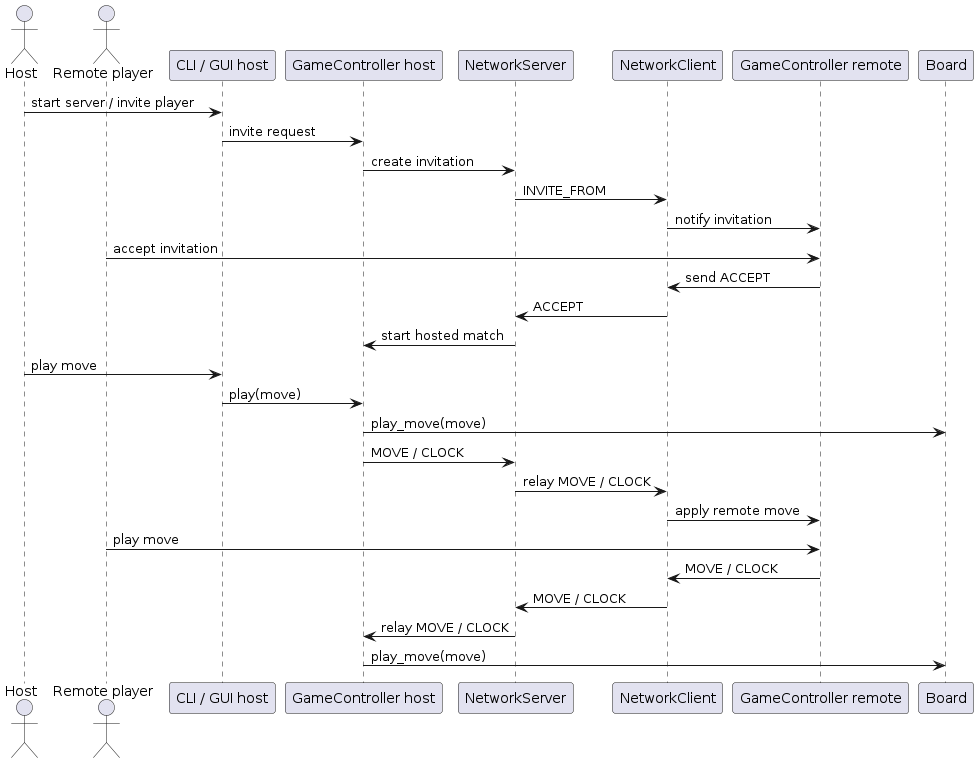
\includegraphics[width=0.95\textwidth]{diag-seq-cli-hh.png}%
  }{%
    \IfFileExists{diag-seq-cli-hh.pdf}{%
      \includegraphics[width=0.95\textwidth]{diag-seq-cli-hh.pdf}%
    }{%
      \fbox{%
        \parbox[c][0.28\textheight][c]{0.82\linewidth}{%
          \centering Ajouter \texttt{diag-seq-cli-hh.png}\\
          ou \texttt{diag-seq-cli-hh.pdf}
        }%
      }%
    }%
  }
  \caption{Séquence : CLI humain vs humain}
  \label{fig:sequence-cli-hh}
\end{figure}

\noindent
Ce diagramme retrace un tour local en CLI entre deux joueurs humains. La vue transmet la commande au \texttt{GameController}. Le contrôleur vérifie le coup, met à jour le plateau et renvoie l'état affiché. Le second joueur suit le même chemin. La CLI sert donc d'interface d'entrée, tandis que la logique reste portée par le contrôleur et le modèle.

\begin{figure}[H]
  \centering
  \IfFileExists{diag-seq-network.png}{%
    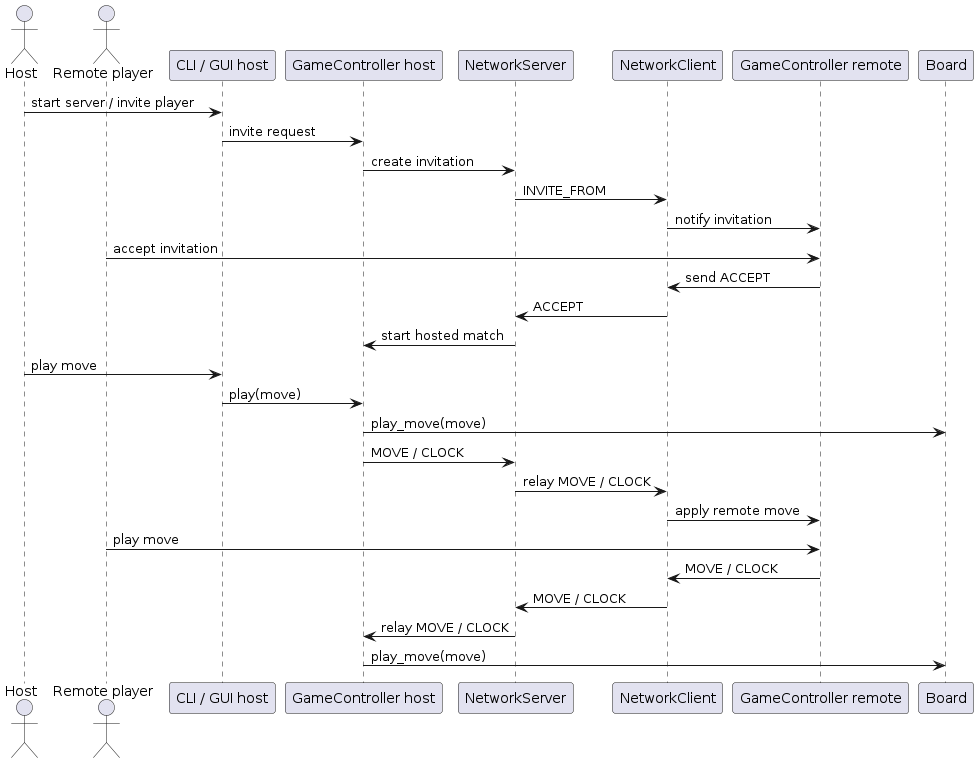
\includegraphics[width=0.95\textwidth]{diag-seq-network.png}%
  }{%
    \IfFileExists{diag-seq-network.pdf}{%
      \includegraphics[width=0.95\textwidth]{diag-seq-network.pdf}%
    }{%
      \fbox{%
        \parbox[c][0.28\textheight][c]{0.82\linewidth}{%
          \centering Ajouter \texttt{diag-seq-network.png}\\
          ou \texttt{diag-seq-network.pdf}
        }%
      }%
    }%
  }
  \caption{Séquence : scénario réseau}
  \label{fig:sequence-network}
\end{figure}

\noindent
La Figure~\ref{fig:sequence-network} montre le même enchaînement lorsqu'un coup vient du réseau. Avant d'atteindre le plateau, le message passe par les composants de découverte, de connexion et de synchronisation. Une fois reçu, il est traité par le \texttt{GameController} comme un coup ordinaire. Le réseau ajoute donc une couche de transport, sans modifier les règles du jeu.

\subsubsection{Architecture réseau}

Le mode réseau repose sur une architecture client--serveur utilisant \texttt{socket} \cite{pythonsocket}, avec séparation explicite entre découverte, connexion persistante et gestion de sessions. Cette séparation évite de confondre l'identification du serveur, l'entrée dans le lobby et la synchronisation stricte d'une partie.

\begin{itemize}
    \item \textbf{Découverte} : broadcast UDP pour localiser le serveur sur le réseau local.
    \item \textbf{Connexion} : canal TCP persistant pour l'échange ordonné des commandes de partie.
    \item \textbf{Lobby} : enregistrement des joueurs connectés, gestion d'identifiants, invitations et état d'attente.
    \item \textbf{Session} : synchronisation d'une partie active, transmission des coups, de l'undo, des événements de fin de partie et mise à jour du scoreboard.
\end{itemize}

Le choix UDP/TCP répond directement au besoin. UDP convient à la découverte : le service doit être visible à faible coût, et la perte d'un paquet reste tolérable. TCP est nécessaire pour la partie elle-même : un coup perdu, dupliqué ou désordonné casserait la cohérence des deux plateaux. Le protocole réseau doit donc être lu comme un mécanisme de synchronisation d'état.

Cette partie correspond directement aux besoins \textbf{F38}, \textbf{F39} et \textbf{F40}. Le contrôleur utilise \texttt{NetworkDiscovery} pour lister les serveurs. Il s'appuie ensuite sur \texttt{NetworkServer} pour accepter plusieurs connexions et sur \texttt{NetworkClient} pour rejoindre une partie existante.

Le protocole repose sur des messages textuels simples, mais il dépasse largement le noyau minimal \texttt{PING}, \texttt{PONG}, \texttt{START}, \texttt{MOVE} et \texttt{QUIT}. Il couvre aussi plusieurs familles d'événements :
\begin{itemize}
    \item notifications de lobby : \texttt{PLAYER\_CONNECTED} ;
    \item invitations : \texttt{INVITE\_*} ;
    \item lancement de partie : \texttt{HOST\_START\_GAME} ;
    \item synchronisation d'horloge : \texttt{CLOCK} ;
    \item undo réseau : \texttt{UNDO\_REQ}, \texttt{UNDO\_OK}, \texttt{UNDO\_NO} ;
    \item fin de partie : \texttt{GAMEOVER} ;
    \item synchronisation de sauvegarde en mode hôte--client : \texttt{LOAD\_STATE}.
\end{itemize}
Ce choix facilite nettement les tests et le débogage, au prix d'un formalisme limité et d'un typage faible des échanges.

\begin{figure}[H]
  \centering
  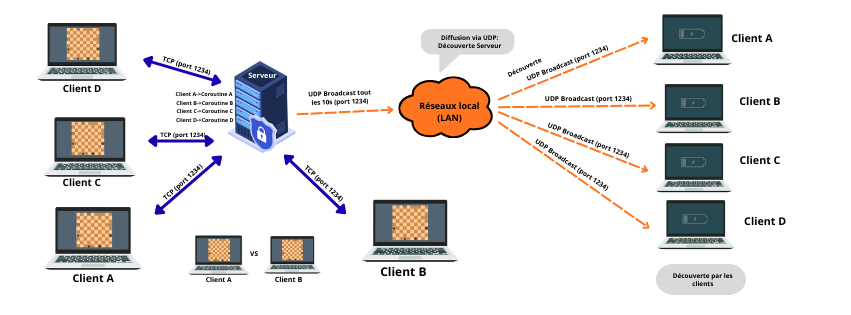
\includegraphics[width=0.92\textwidth]{shema_reseaux.png}
  \caption{Architecture réseau client-serveur}\label{fig:reseau}
\end{figure}

Ce schéma représente le flux de communication entre découverte, connexion et partie effective. Il illustre un choix architectural important : la couche réseau s'ajoute au moteur existant sans le remplacer. La validation des coups reste locale au moteur, tandis que le réseau transporte des intentions et des états synchronisés. Cette approche réduit le risque de divergence de règles entre mode local et mode distant, mais elle impose une vigilance particulière sur la synchronisation des états.

L'architecture actuelle est plus riche qu'un schéma client unique contre serveur. Le serveur maintient un lobby multi-clients, des invitations, un joueur hôte, des sessions actives entre deux clients ou entre l'hôte et un client, ainsi qu'un scoreboard persistant pendant la durée de vie du serveur. Cette dimension est importante à expliciter dans le rapport : elle montre que le système réseau ne se limite pas à transférer des coups, mais gère aussi un cycle de vie de partie, des rôles, des transitions d'état et des déconnexions. En outre, le code distingue explicitement deux cas d'usage : les matchs \emph{hosted} (hôte contre client) et les matchs \emph{relayed} (client contre client via le serveur), qui n'autorisent pas exactement les mêmes opérations, notamment pour la synchronisation de sauvegarde.

Cette synchronisation constitue d'ailleurs l'une des limites structurelles du projet. Le réseau est traité selon un modèle principalement synchrone côté contrôleur, alors que la GUI introduit naturellement une logique événementielle et asynchrone. Cette tension entre boucles bloquantes de type CLI et callbacks graphiques rend la conception plus fragile qu'un système entièrement événementiel. Dans une version industrielle, on privilégierait probablement un protocole de messages typés et une couche d'orchestration asynchrone explicitement séparée de la logique métier.

\subsubsection{Intégration des fonctionnalités avancées}

La liste complète des quarante besoins figure en annexe. Dans le corps du rapport, nous montrons surtout comment les fonctionnalités avancées reposent sur le même noyau technique.

\begin{itemize}
    \item Les bitboards et la génération de coups forment le socle commun du moteur.
    \item Les moteurs d'IA réutilisent directement \texttt{Board}, \texttt{Move} et les opérations de jeu.
    \item Le réseau transporte des commandes et des états synchronisés, mais ne redéfinit pas les règles.
    \item La GUI pilote le même contrôleur et les mêmes objets métier que la CLI.
    \item La persistance reconstruit ce même état, ce qui évite de multiplier les formats et les chemins de traitement.
\end{itemize}

Cette organisation explique pourquoi le projet reste cohérent malgré la diversité des modes d'utilisation. Les fonctionnalités avancées ne contournent pas le moteur central ; elles l'exploitent et l'étendent.

\subsubsection{Internationalisation}

Le projet supporte l'anglais (par défaut) et le français via \texttt{gettext} \cite{gettext2024}. La langue peut être imposée au lancement ou déduite de la locale système. Les catalogues sont rangés dans \texttt{locales/en/} et \texttt{locales/fr/}. Ce choix garde la traduction dans un service transversal au lieu de la disperser dans les modules métier.

\subsection{Préoccupation de qualité logicielle}

Dès la phase de conception, une attention particulière a été portée à la testabilité et à la cohérence des composants. Le moteur de jeu, la persistance, les services réseau et les vues ont été séparés autant que possible afin de limiter les dépendances circulaires et de faciliter la validation ultérieure. Cette préoccupation explique notamment le rôle des services transversaux comme \texttt{SaveLoadManager} et l'importance donnée à des interfaces stables entre le contrôleur, le plateau et les différents types de joueurs.

Cette logique de qualité ne supprime pas les défauts du système. Elle aide surtout à lire les choix faits dans le projet : compromis entre extensibilité, délai de réalisation, lisibilité et performance.

\paragraph{Synthèse des décisions d'ingénierie.}
\begin{table}[H]
\centering
\begin{tabular}{p{3.2cm} p{5.2cm} p{5.2cm}}
\toprule
\textbf{Décision} & \textbf{Gain principal} & \textbf{Coût ou dette associée} \\
\midrule
Bitboards & Représentation compacte, tests d'occupation rapides, bonne adéquation au moteur et à l'IA & Lisibilité plus faible qu'une matrice 2D, indexation plus abstraite \\
Coexistence Minimax / MCTS & Comparaison de stratégies de décision complémentaires sous une API commune & Maintenance plus exigeante, réglages d'heuristiques multiples \\
Contrôleur central & Intégration rapide des fonctionnalités transversales & Concentration des responsabilités et maintenabilité réduite \\
Protocole réseau textuel & Débogage simple, inspection aisée des échanges & Typage faible, validation plus fragile qu'avec des messages structurés \\
\bottomrule
\end{tabular}
\caption{Synthèse des décisions d'ingénierie structurantes du projet.}
\label{tab:engineering-decisions}
\end{table}

%==============================================================================
%   SECTION 4 : EXPLICATION APPROFONDIE DE DEUX FONCTIONNALITÉS
%==============================================================================

\section{Explication approfondie}
\label{sec:explication-approfondie}

Cette section isole deux fonctionnalités effectivement réalisées et centrales dans le projet. Le choix retenu n'est pas arbitraire : la génération des coups bitboard constitue le noyau fonctionnel du moteur, tandis que Minimax avec élagage $\alpha\beta$ est le moteur d'IA le plus directement explicable et le mieux intégré au code actuel.

\subsection{Fonctionnalité 1 --- Génération des coups avec bitboards}

\paragraph{Objectif.}
Produire tous les coups légaux d'un joueur sous la forme \texttt{Move(start, end, arrow)}. Cette fonctionnalité est partagée par le moteur, la validation locale, les IA et le contrôleur ; une erreur ici affecte donc immédiatement tout le système.

\paragraph{Conception.}
Le code s'appuie sur trois bitboards spécialisés et sur une occupation agrégée \texttt{occupied}. Les amazones du joueur sont extraites une par une via le bit de poids faible, puis le même itérateur de déplacement de reine est réutilisé deux fois : d'abord pour les destinations de déplacement, puis pour les cibles de flèche après reconstruction d'une occupation temporaire.

\paragraph{Algorithme détaillé.}
Entrée : la couleur à jouer et l'état courant du plateau. Sortie : un flux de coups complets.

Pour le coup \texttt{e2-e4/e6}, l'exécution suit exactement les étapes suivantes :
\begin{enumerate}
    \item sélectionner l'amazone de départ \texttt{e2} ;
    \item propager dans la direction choisie en contrôlant à chaque pas les bornes ligne/colonne et l'absence de collision ;
    \item retenir \texttt{e4} seulement si le chemin \texttt{e2} $\rightarrow$ \texttt{e4} est libre ;
    \item reconstruire \texttt{occupied\_after\_move} en retirant \texttt{e2} puis en occupant \texttt{e4} ;
    \item relancer exactement le même itérateur depuis \texttt{e4} pour les tirs de flèche ;
    \item retenir \texttt{e6} seulement si cette seconde trajectoire est libre ;
    \item produire finalement \texttt{Move(e2, e4, e6)}.
\end{enumerate}

Le \textit{wrapping} est évité par le contrôle explicite de \texttt{row} et \texttt{col} avant reconstruction de l'index. L'occupation intervient donc deux fois : d'abord pour filtrer les destinations, puis sous forme modifiée pour filtrer les cases de flèche.

\paragraph{Déroulement technique.}
L'implémentation repose sur deux boucles imbriquées de propagation. La première parcourt toutes les destinations atteignables depuis une amazone donnée dans l'occupation courante. La seconde repart de chaque destination candidate avec une occupation recalculée, où la case de départ est redevenue libre et la case d'arrivée est désormais occupée. Cette mise à jour intermédiaire est le point décisif de la fonction : elle évite d'accepter un tir de flèche à travers l'amazone déplacée, tout en autorisant un tir sur l'ancienne case de départ lorsque les règles le permettent. La sortie finale n'est donc pas une simple liste de destinations, mais un ensemble de triplets complets \texttt{(départ, arrivée, flèche)} déjà compatibles avec l'état réel du plateau après déplacement.

\paragraph{Intégration dans le système.}
Cette fonctionnalité est fournie par \texttt{Board.get\_legal\_moves(color)}. Elle est utilisée directement par \texttt{Board.is\_valid\_move}, par \texttt{MinimaxEngine} et \texttt{MCTSEngine}, et indirectement par le contrôleur lorsqu'il doit décider si un joueur peut encore jouer.

\paragraph{Tests associés.}
Les tests vérifient notamment qu'un coup bloqué n'est pas produit, qu'un déplacement en bord de plateau n'induit pas de \textit{wrapping}, qu'un coup généré puis annulé restaure exactement les trois bitboards, et que l'ancienne case de départ peut devenir une cible de flèche après libération.

\subsection{Fonctionnalité 2 --- IA Minimax avec élagage \texorpdfstring{$\alpha\beta$}{alpha-beta}}

\paragraph{Objectif.}
Choisir un coup légal de bonne qualité sous contrainte de profondeur et de temps. Dans le projet, ce moteur sert de base déterministe pour l'IA et de référence pour comparer le comportement de MCTS.

\paragraph{Conception.}
\texttt{AIPlayer} ne réalise pas lui-même la recherche. Il instancie \texttt{MinimaxEngine} selon le mode demandé, puis lui transmet le plateau et la couleur du joueur. Le moteur réutilise directement les primitives du plateau : génération des coups, application, annulation et évaluation heuristique.

\paragraph{Algorithme détaillé.}
La méthode \texttt{best\_move(board, color)} matérialise d'abord tous les coups légaux du joueur courant. Pour chaque coup candidat, elle :
\begin{enumerate}
    \item applique le coup via \texttt{board.play\_move(move)} ;
    \item appelle récursivement \texttt{minimax(...)} avec alternance MAX/MIN ;
    \item coupe une branche si $\alpha \geq \beta$ ;
    \item restaure l'état exact via \texttt{board.undo\_move(move, color)} ;
    \item conserve le coup associé au meilleur score.
\end{enumerate}

La récursion s'arrête dans trois cas : profondeur nulle, absence de coups légaux pour le joueur courant, ou dépassement du budget temps. Dans les feuilles, le score provient de \texttt{Evaluator.evaluate(board, color, mode)}.

\paragraph{Déroulement technique.}
Le moteur commence par figer l'ensemble des coups légaux du joueur courant, puis les évalue un par un dans une boucle principale. Chaque itération suit le même cycle : appliquer le coup sur le plateau partagé, lancer l'exploration récursive avec alternance MAX/MIN, mettre à jour les bornes $\alpha$ et $\beta$, puis restaurer immédiatement l'état exact du plateau. Le meilleur coup n'est conservé qu'après cette restauration, ce qui garantit que l'itération suivante repart d'un état propre. Dans le code, cette discipline \og appliquer, explorer, annuler \fg{} est essentielle : elle évite la copie systématique du plateau, garde la mémoire sous contrôle et permet d'utiliser le même moteur sur tous les états produits par le contrôleur.

\paragraph{Intégration dans le système.}
Le couplage avec le reste du projet reste simple. \texttt{AIPlayer.get\_action(...)} construit le moteur. \texttt{MinimaxEngine.best\_move(...)} interroge ensuite \texttt{Board}. Le coup retenu est renvoyé au contrôleur comme un coup humain. Le contrôleur n'a donc pas besoin de connaître la stratégie interne du moteur.

\paragraph{Limites concrètes et comportement observé.}
Ce moteur est fiable et reproductible, mais il souffre rapidement de l'explosion combinatoire. Les mesures du rapport montrent déjà qu'à profondeur 2, les grands plateaux sortent du cadre interactif. En pratique, Minimax reste donc pertinent pour des profondeurs modestes, pour l'approfondissement itératif et pour des scénarios où l'on veut une décision explicable par une heuristique.

\paragraph{Tests associés.}
Les tests associés vérifient qu'un coup renvoyé par Minimax appartient bien à l'ensemble des coups légaux, qu'un plateau sans coup légal renvoie \texttt{None}, que le moteur reste borné par le budget temps, et que l'appel à \texttt{best\_move} ne corrompt pas durablement l'état du plateau grâce au couple \texttt{play\_move}/\texttt{undo\_move}.

\section{Implémentation}

\subsection{Moteur de jeu et structures internes}

\subsubsection{Représentation mémoire}

En Python, les entiers sont de précision arbitraire, ce qui permet de représenter un plateau allant jusqu'à $11 \times 11 = 121$ cases dans une seule valeur entière. Le moteur maintient trois bitboards spécialisés : un pour les amazones blanches, un pour les amazones noires et un pour les flèches. Cette séparation est un invariant central du modèle : un bitboard ne mélange jamais plusieurs types d'objets.

L'occupation totale est calculée par une simple opération OR :
\[
\texttt{occupied} = \texttt{white\_bb} \mid \texttt{black\_bb} \mid \texttt{arrow\_bb}
\]

Ce choix a deux effets directs sur le moteur. D'abord, tester une case coûte une seule opération binaire : on forme le masque \texttt{1 << pos}, puis on vérifie \texttt{occupied \& mask}. Ensuite, déplacer une amazone ou poser une flèche revient à modifier quelques bits dans les trois bitboards, sans recopier un tableau complet. C'est exactement le type d'opération répété par \texttt{get\_legal\_moves}, \texttt{play\_move}, \texttt{undo\_move} et les moteurs d'IA.

L'exemple de \texttt{d4} sur un plateau $10 \times 10$ rend cela concret. Le code numérote les cases en \textit{row-major} depuis le coin supérieur gauche ; \texttt{d4} correspond donc à la colonne 3 et à la ligne interne 6, soit l'index \texttt{63}. Le masque \texttt{1 << 63} pointe exactement cette case. On peut alors tester son occupation via \texttt{occupied \& (1 << 63)}, l'activer via \texttt{bitboard | (1 << 63)} et la désactiver par \texttt{XOR} si le bit est déjà actif. Le gain n'est donc pas limité à la mémoire : une case devient une cible binaire que le moteur manipule directement.

\subsubsection{Génération des coups légaux --- Implémentation détaillée}

\texttt{get\_legal\_moves(color)} reprend la logique détaillée dans la Section~\ref{sec:explication-approfondie}. Ici, le point important est son rôle central : validation, IA et détection de fin de partie reposent sur cette même méthode.

\subsubsection{Application et annulation de coups}

L'application d'un coup modifie directement les bitboards via \texttt{XOR} et \texttt{OR} : retrait de l'amazone sur la case de départ, activation de la case d'arrivée, puis ajout de la flèche. L'annulation suit l'ordre inverse. Cet ordre garantit notamment qu'une flèche peut retomber légalement sur l'ancienne case de l'amazone si elle est redevenue libre au bon moment.

\subsubsection{Validation des coordonnées}

La conversion algébrique $\rightarrow$ index inclut une validation stricte des bornes pour prévenir les erreurs silencieuses. Le moteur sépare le calcul de la colonne, le calcul de la ligne et le contrôle de compatibilité avec la taille du plateau. En cas d'entrée invalide, il lève explicitement une exception plutôt que de corriger ou d'ignorer la valeur, ce qui protège la CLI, la GUI et le chargement de parties contre les coordonnées incohérentes.

% ----- Fonctionnalité 2 -----

\subsection{Implémentation de l'intelligence artificielle}

L'intelligence artificielle du jeu repose sur plusieurs stratégies complémentaires, sélectionnées explicitement dans le code en fonction du mode choisi pour le joueur.

\subsubsection{Architecture de l'IA}

Le joueur IA (\texttt{AIPlayer}) ne contient pas lui-même les algorithmes de recherche. Il choisit un moteur selon le mode configuré (\texttt{random}, \texttt{minimax}, \texttt{iterative}, \texttt{mcts}) et lui délègue la production du coup. Le terme \og hybride \fg{} désigne ici l'évaluateur, pas un moteur combinant directement Minimax et MCTS. L'option \texttt{ML} visible dans le lancement n'est pas encore reliée à un moteur d'apprentissage réel.

\subsubsection{Sélection du moteur}

Ce \textit{dispatch} simplifie l'ajout futur de nouveaux moteurs et évite d'exposer au contrôleur des détails propres à Minimax ou à MCTS.

\subsubsection{Implémentation Minimax avec élagage \texorpdfstring{$\alpha\beta$}{alpha-beta}}

Dans le code, \texttt{MinimaxEngine.best\_move} itère sur les coups produits par \texttt{board.get\_legal\_moves(color)}, applique chaque coup, appelle \texttt{minimax(...)} puis restaure l'état avec \texttt{board.undo\_move(move, color)}. Le détail algorithmique et les scénarios de test sont donnés dans la Section~\ref{sec:explication-approfondie}. Le point d'implémentation utile ici est l'absence de copie complète du plateau à chaque nœud : le moteur réutilise le même objet \texttt{Board} par application et annulation successives.

\subsubsection{Implémentation MCTS}

Le MCTS \cite{browne2012mcts} est particulièrement adapté aux jeux à grand facteur de branchement comme les Amazones. Chaque nœud mémorise le joueur à traiter, le coup ayant conduit à ce nœud, le nombre de visites, le nombre de simulations gagnantes, les enfants déjà explorés et les coups encore inexplorés.

La sélection d'un enfant s'appuie sur une variante de UCT. Le code stocke les victoires du point de vue du joueur du nœud enfant. Pour choisir depuis le parent, il convertit donc ce score en taux de succès du parent, puis ajoute le terme d'exploration classique. Ce détail est important : il explique pourquoi la formule du code n'est pas écrite exactement comme la version canonique des articles.

La boucle MCTS s'exécute pendant le budget temps alloué :

\begin{enumerate}
    \item \textbf{Sélection} : descendre en choisissant le fils avec le meilleur UCT.
    \item \textbf{Expansion} : ajouter un fils non exploré.
    \item \textbf{Simulation} : partie aléatoire jusqu'à la fin (rollout).
    \item \textbf{Rétropropagation} : mettre à jour wins et visits sur tout le chemin.
\end{enumerate}

Le point essentiel d'implémentation est le suivant : les nœuds MCTS ne conservent pas de copie complète du plateau. Le moteur reconstruit un état de travail à partir du plateau racine et rejoue les coups au fil de l'itération. Ce choix réduit la pression mémoire, au prix d'un surcoût de recomputation.

\subsubsection{Approfondissement itératif et budget temps}

En plus de Minimax et MCTS, le projet inclut une stratégie d'\textbf{approfondissement itératif}. Le principe consiste à lancer successivement des recherches Minimax de profondeur croissante tant que le budget temps n'est pas épuisé. Cette approche présente deux avantages concrets :

\begin{itemize}
    \item elle garantit qu'un \textbf{meilleur coup connu} est toujours disponible, même si le temps est écoulé brutalement ;
    \item elle permet d'utiliser efficacement le temps disponible sans fixer à l'avance une profondeur trop ambitieuse ou trop conservatrice.
\end{itemize}

Cette stratégie améliore la robustesse pratique du moteur sur les grands plateaux tout en restant compatible avec les budgets temps imposés au joueur artificiel.

\subsubsection{Évaluateur territorial (BFS)}

L'évaluateur de territoire, inspiré de Lieberum \cite{lieberum1999}, repose dans notre version sur une propagation locale depuis toutes les amazones d'un joueur, en voisinage de roi, à travers les cases libres. Il ne cherche donc pas encore à calculer une véritable compétition de distances minimales entre les deux camps ; il mesure plutôt l'étendue des zones encore atteignables sans traverser les obstacles. Cette approximation reste intéressante car elle capte déjà la structure spatiale du plateau pour un coût raisonnable, mais elle doit être comprise comme une heuristique d'ingénierie et non comme une modélisation exacte du contrôle territorial.

\subsubsection{Gestion du temps}

L'IA dispose d'un budget temps configurable (\texttt{-{}-ai-time}, défaut 5s). Le Minimax avec approfondissement itératif augmente progressivement la profondeur tant que le temps le permet, ce qui garantit qu'un coup valide reste toujours disponible. Le MCTS, lui, s'arrête naturellement quand le budget est épuisé.

% ----- Persistance et interfaces -----

\subsection{Persistance, interfaces et intégration}

\subsubsection{Sauvegarde et chargement des parties}

Le service de persistance repose sur un format ASCII structuré en sections. Un fichier de sauvegarde contient les paramètres de partie, l'état du plateau, l'historique des coups et, lorsque cela s'applique, un checksum. Ce choix garde le format lisible, facile à déboguer et indépendant d'un format binaire opaque.

Le chargeur accepte des commentaires en ligne (\texttt{\# ...}) et des commentaires de bloc (\texttt{\{ ... \}}), reconstruit le plateau à partir des symboles sérialisés, recharge l'historique en notation algébrique, puis vérifie la cohérence logique de l'état obtenu. Il peut aussi adapter la taille du contrôleur si la taille lue dans le fichier diffère de l'état courant. Enfin, la synchronisation réseau d'une sauvegarde chargée n'est prise en charge que dans les parties hôte--client ; elle n'est pas autorisée dans les parties client--client relayées.

L'implémentation sépare la sérialisation, la validation du contenu et la reconstruction de l'état. Charger une partie ne revient donc pas à lire un fichier : il faut aussi vérifier que le contenu décrit bien un état de jeu cohérent.

\subsubsection{Intégration de la GUI}

L'interface graphique GTK4 réutilise le même noyau métier que la CLI. Elle n'interprète pas elle-même les règles du jeu : elle transmet des intentions d'action au contrôleur, qui reste responsable de la validation, de l'application des coups et de la mise à jour de l'état. Ce choix limite les duplications de logique et facilite la cohérence entre les deux interfaces.

Sur le plan utilisateur, la GUI offre une lecture plus directe du plateau, des menus de configuration et des actions de sauvegarde ou de chargement. Les captures retenues dans le rapport ont été volontairement simplifiées : elles ne montrent que le plateau, l'indication du joueur courant et les marqueurs utiles au tour. L'icône de reine y représente une amazone ; le contour bleu désigne l'amazone actuellement sélectionnée ; les points noirs indiquent les cases légales de déplacement ou de tir selon la phase en cours. Cette convention rend la lecture des figures autonome, même pour un lecteur qui ne connaît pas encore l'interface.

Sur le plan logiciel, la GUI reste une vue branchée sur les mêmes objets métier. L'implémentation actuelle va toutefois au-delà d'un simple affichage local : \texttt{gui\_config.py} porte la configuration réseau et le lobby hôte, \texttt{gui\_menu.py} les actions de menus et de sauvegarde/chargement, et \texttt{gui\_shortcuts.py} les raccourcis. La GUI gère aujourd'hui des matchs locaux, des matchs hôte contre client, un lobby multi-clients avec invitations, l'affichage du scoreboard, et le lancement d'une partie client contre client relayée par le serveur. Sa maturité reste toutefois inégale selon les scénarios, en particulier du côté de l'ergonomie et de la validation automatique.

\begin{figure}[H]
\centering
\begin{minipage}[t]{0.32\textwidth}
\centering
\annotatedturnshot{tour_1_selection.png}{Capture 1 : sélection d'une reine}{%
  \draw[red, rounded corners=2pt, line width=1.6pt]
    (0.26,0.77) rectangle (0.40,0.96);
}

\small (a) \texttt{Player1} est le joueur actif ; l'amazone claire entourée en bleu lui appartient et les points noirs marquent ses destinations atteignables.
\end{minipage}\hfill
\begin{minipage}[t]{0.32\textwidth}
\centering
\annotatedturnshot{tour_2_deplacement.png}{Capture 2 : déplacement de l'amazone}{%
  \draw[red, rounded corners=2pt, line width=1.6pt]
    (0.27,0.60) rectangle (0.40,0.75);
}

\small (b) Après le déplacement, la même amazone reste la pièce active et l'interface passe à la phase de tir.
\end{minipage}\hfill
\begin{minipage}[t]{0.32\textwidth}
\centering
\annotatedturnshot{tour_3_fleche.png}{Capture 3 : tir de la flèche}{%
  \draw[red, rounded corners=2pt, line width=1.6pt]
    (0.43,0.45) rectangle (0.58,0.58);
}

\small (c) La flèche est posée, la case devient bloquée, puis le tour passe à \texttt{Player2}, représenté par les amazones sombres.
\end{minipage}
\caption{Déroulement d'un tour dans l'interface graphique : sélection d'une amazone du joueur courant, déplacement, puis tir de flèche.}
\label{fig:gui-turn}
\end{figure}

\subsubsection{Intégration du réseau}

Le réseau a été implémenté comme un service additionnel, et non comme une logique parallèle au moteur. Les messages reçus à distance sont convertis vers les mêmes objets et les mêmes opérations que dans une partie locale. Cette stratégie a deux avantages : elle limite les divergences entre modes de jeu et elle permet de conserver une unique source de vérité pour la validation des coups.

%==============================================================================
%   SECTION 7 : TESTS ET VALIDATION
%==============================================================================

\section{Tests et validation}

La validation du projet combine tests automatisés, vérifications manuelles ciblées et essais en situation réelle. Cette approche est nécessaire : le moteur bitboard et le chargeur de sauvegardes se testent bien unitairement, alors que la GUI et certains scénarios réseau demandent encore des vérifications interactives. Le but est de vérifier que les invariants tiennent quand on combine moteur, interfaces, IA et persistance.

\subsection{Stratégie de test}

Le Tableau~\ref{tab:test-strategy} résume le mode de validation privilégié pour chaque grand composant du projet. Il sert surtout à distinguer ce qui relève de tests automatisés stables et ce qui relève encore d'essais guidés.

\begin{table}[H]
\centering
\begin{tabular}{lp{9cm}}
\toprule
\textbf{Composant} & \textbf{Mode de validation privilégié} \\
\midrule
Moteur bitboard & tests unitaires sur la génération, l'application et l'annulation des coups \\
Persistance & scénarios de sauvegarde/chargement, validations de format et de checksum \\
CLI et contrôleur & tests d'intégration sur les commandes, l'historique et les transitions de tour \\
IA & scénarios de sélection de coup, évaluateurs et budgets temps \\
Réseau et GUI & tests manuels guidés et essais de cohérence fonctionnelle \\
\bottomrule
\end{tabular}
\caption{Répartition des stratégies de validation selon les composants.}
\label{tab:test-strategy}
\end{table}

Le moteur bitboard est le composant le plus simple à valider automatiquement, car il expose des invariants nets : un coup légal doit être généré, appliqué puis annulé sans corrompre l'état. La persistance est validée de la même manière, en reconstruisant des parties sérialisées puis en vérifiant la cohérence logique de l'état restauré. Des scénarios typiques consistent par exemple à jouer un coup, l'annuler, puis vérifier que les trois bitboards retrouvent exactement leur état initial, ou à charger une sauvegarde contenant une coordonnée invalide et vérifier que le chargeur la rejette explicitement.

La CLI et le contrôleur nécessitent une approche plus intégrative. Les tests portent sur des transitions complètes : lecture d'une commande, validation, mise à jour du plateau, gestion de l'historique et retour utilisateur. Enfin, le réseau et la GUI restent les zones les plus coûteuses à automatiser complètement, car ils dépendent d'événements asynchrones, de l'interface graphique et de la synchronisation de plusieurs acteurs ; ils sont donc encore validés en partie par des scénarios manuels guidés, comme la création d'un lobby, l'invitation d'un client, l'envoi d'un coup, une demande d'undo ou le chargement d'une sauvegarde en mode hôte--client.

\subsection{Outils et critères de validation}

Le projet utilise \texttt{pytest} \cite{pytest2024} pour automatiser une partie importante des validations, complété par des vérifications manuelles ciblées sur les scénarios GUI et réseau. Au moment de la rédaction, la suite contient \textbf{470 tests réussis} et la couverture mesurée atteint \textbf{86\,\%} sur le paquet \texttt{amazons}. Trois niveaux de validation doivent être distingués.

Le premier niveau est la \textbf{validation fonctionnelle locale}. Il concerne le moteur, la génération des coups, l'application et l'annulation, les conversions de notation et la persistance. À ce niveau, la vraie question est simple : le système préserve-t-il les invariants du jeu ? C'est ici que les tests unitaires ont le plus de valeur.

Le deuxième niveau est la \textbf{validation d'intégration}. Elle concerne les interactions entre modules : par exemple, vérifier qu'une commande CLI déclenche bien une transition cohérente dans le contrôleur, qu'une sauvegarde reconstruite correspond à un état jouable, ou qu'une IA produit un coup exploitable par le moteur sans corrompre l'historique. Ce niveau est déterminant car le projet repose sur un noyau métier partagé entre plusieurs points d'entrée.

Le troisième niveau est la \textbf{validation système}. Elle cible les scénarios où plusieurs couches interagissent simultanément : partie réseau, chronométrage, invitations, GUI et synchronisation d'état. C'est également le niveau le plus difficile à automatiser complètement, car il dépend d'événements asynchrones et d'interactions utilisateur.

Les chiffres de tests doivent donc être lus avec prudence. Un grand nombre de tests réussis rassure sur le noyau, mais ne garantit pas à lui seul la stabilité de toutes les interactions entre interfaces. La validation doit être jugée sur les risques réellement couverts, pas sur le nombre de tests seul.

%==============================================================================
%   SECTION 8 : ANALYSE DE PERFORMANCES
%==============================================================================

\section{Analyse de performances}

Cette section relie quelques mesures simples aux choix algorithmiques du projet. L'objectif n'est pas de produire un benchmark industriel, mais d'illustrer la croissance du facteur de branchement, la sensibilité de Minimax à la profondeur et le comportement \emph{anytime} de MCTS.

\subsection{Mesures}

\begin{table}[H]
\centering
\small
\begin{tabular}{ccccc}
\toprule
\textbf{Taille} & \textbf{Coups initiaux} & \textbf{Minimax $d=1$} & \textbf{Minimax $d=2$} & \textbf{MCTS $0{,}5$s} \\
\midrule
$4 \times 4$ & 104 & $0{,}013\,s$ & $0{,}820\,s$ & $0{,}500\,s$ \\
$5 \times 5$ & 198 & $0{,}045\,s$ & $7{,}083\,s$ & $0{,}501\,s$ \\
$6 \times 6$ & 496 & $0{,}242\,s$ & $> 20\,s$ & $0{,}502\,s$ \\
$8 \times 8$ & 1232 & $1{,}359\,s$ & $> 20\,s$ & $0{,}503\,s$ \\
$10 \times 10$ & 2176 & $4{,}218\,s$ & $> 20\,s$ & $0{,}510\,s$ \\
\bottomrule
\end{tabular}
\caption{Mesures sur la position initiale : croissance du facteur de branchement et temps de décision.}
\label{tab:benchmarks}
\end{table}

Le premier résultat marquant est l'augmentation rapide du nombre de coups légaux. On passe de 104 coups sur un plateau $4 \times 4$ à 2176 coups sur un plateau $10 \times 10$. Cette croissance explique directement pourquoi les recherches adversariales profondes deviennent vite difficiles à maintenir interactives.

Le deuxième résultat concerne Minimax. À profondeur 1, le moteur reste utilisable sur les petits plateaux, mais dépasse déjà 4 secondes sur la position initiale standard. À profondeur 2, le temps de calcul explose : le plateau $5 \times 5$ dépasse 7 secondes et les tailles supérieures dépassent 20 secondes. Cette évolution illustre concrètement la complexité en $O(b^d)$ : dès que le facteur de branchement $b$ devient grand, une faible augmentation de profondeur rend la recherche non interactive. La raison est simple : à chaque nœud, Minimax doit régénérer de très nombreux coups, explorer leurs successeurs et répéter ce travail récursivement.

Le troisième résultat concerne MCTS. Avec un budget de $0{,}5$ seconde, le temps de réponse reste stable quelle que soit la taille du plateau. Ce comportement ne signifie pas que le problème devient facile ; il montre que le moteur respecte d'abord une contrainte de temps, puis améliore sa décision à l'intérieur de ce budget. MCTS utilise donc mieux le temps disponible, car sa boucle s'arrête naturellement à l'échéance au lieu de viser une profondeur fixe qui devient vite hors de portée.

\subsection{Comparaison expérimentale des IA}

Pour compléter les mesures précédentes, nous avons exécuté le script \texttt{scripts/benchmark\_ai.py} sur deux confrontations courtes. Le script alterne les couleurs d'une partie à l'autre, ce qui évite de confondre l'effet du moteur avec l'avantage éventuel du trait. La Figure~\ref{fig:benchmark-ia} montre les deux sorties retenues : \texttt{minimax} contre \texttt{mcts} sur plateau $6 \times 6$, puis \texttt{minimax} contre \texttt{random} sur plateau $10 \times 10$.

\begin{figure}[H]
\centering
\begin{minipage}[t]{0.49\linewidth}
\centering
\textbf{(a) Minimax vs MCTS sur $6 \times 6$}\\[0.25em]
\IfFileExists{benchmark_minimax_mcts.png}{%
  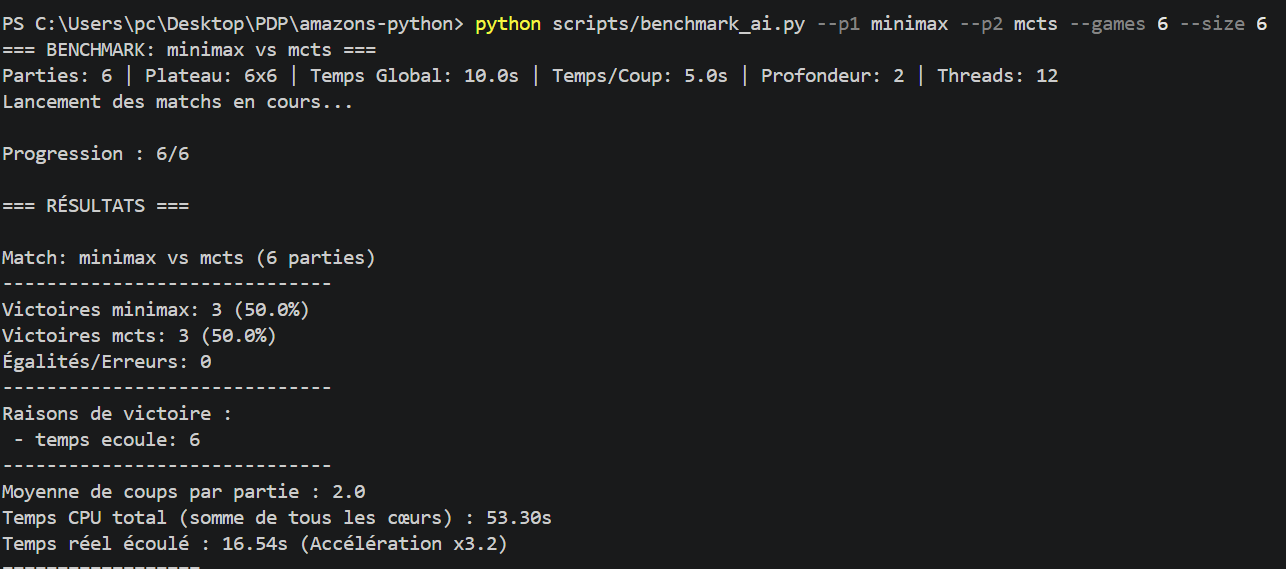
\includegraphics[width=\linewidth]{benchmark_minimax_mcts.png}%
}{%
  \fbox{\parbox[c][0.12\textheight][c]{0.92\linewidth}{\centering Ajouter \texttt{benchmark\_minimax\_mcts.png}}}%
}
\end{minipage}
\hfill
\begin{minipage}[t]{0.49\linewidth}
\centering
\textbf{(b) Minimax vs Random sur $10 \times 10$}\\[0.25em]
\IfFileExists{benchmark_minimax_random.png}{%
  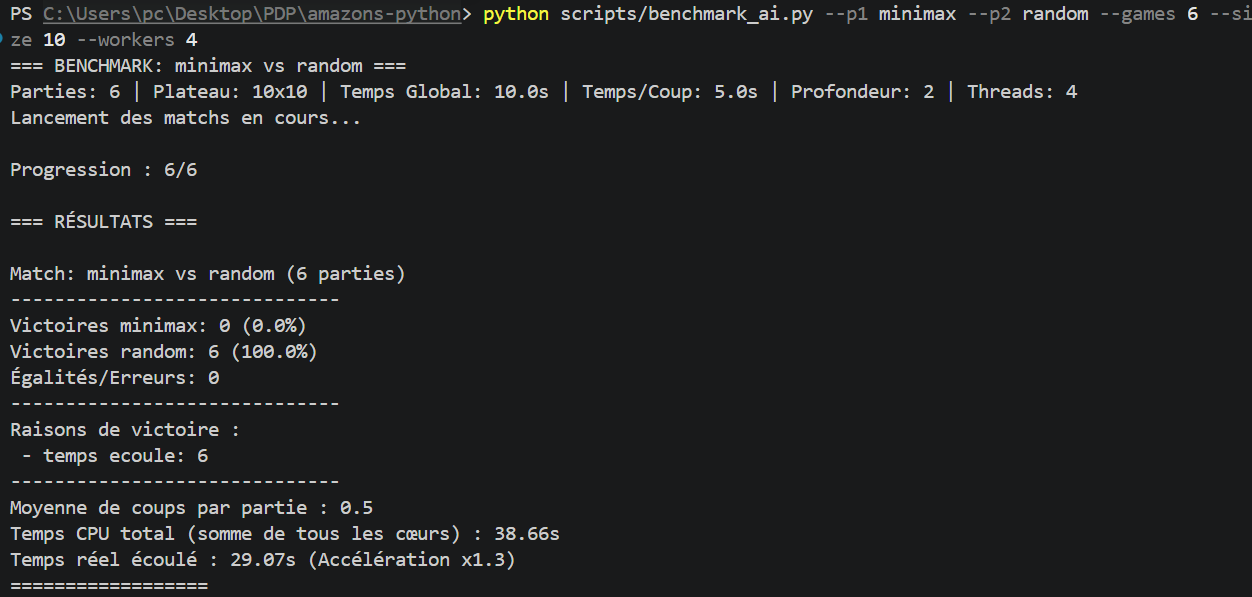
\includegraphics[width=\linewidth]{benchmark_minimax_random.png}%
}{%
  \fbox{\parbox[c][0.12\textheight][c]{0.92\linewidth}{\centering Ajouter \texttt{benchmark\_minimax\_random.png}}}%
}
\end{minipage}
\caption{Captures du benchmark expérimental des IA : 6 parties, couleurs alternées, profondeur Minimax 2, budget de 5 secondes par coup et 10 secondes par joueur.}
\label{fig:benchmark-ia}
\end{figure}

Le premier résultat est un équilibre apparent : sur six parties, \texttt{minimax} et \texttt{mcts} gagnent chacun trois fois. Ce $50/50$ ne prouve pas que les deux moteurs se valent en général. Il reflète surtout ce réglage précis : un échantillon très court, un plateau $6 \times 6$ où la profondeur 2 reste encore jouable pour Minimax, et un budget temps trop faible pour que MCTS stabilise vraiment ses statistiques. Dans ces conditions, aucun moteur ne prend un avantage net.

Le comportement des deux IA reste pourtant différent. Minimax est déterministe : à plateau et paramètres identiques, il parcourt les coups dans le même ordre et applique la même heuristique. Ses décisions sont stables, mais leur qualité dépend directement de la profondeur atteinte. MCTS est plus exploratoire : la sélection suit UCT, puis la simulation repose sur des coups aléatoires. Il peut trouver de bons coups sans profondeur fixe, mais il reste moins stable d'une partie à l'autre.

Le second résultat est plus utile que surprenant : \texttt{random} gagne les six parties face à \texttt{minimax} sur plateau $10 \times 10$, et les six victoires sont comptées pour \og temps écoulé \fg{}. Le benchmark ne dit donc pas que \texttt{random} joue mieux. Il montre qu'avec profondeur 2 et 5 secondes par coup, Minimax dépasse le budget sur grand plateau, alors que \texttt{random} répond presque immédiatement. Dans cette expérience, on mesure d'abord la tenue d'un moteur sous contrainte de temps.

Au vu de ces essais, Minimax reste adapté aux petits et moyens plateaux, ou aux cas où l'on veut une décision stable et explicable. MCTS devient plus crédible dès que le facteur de branchement monte et qu'il faut surtout garantir une réponse dans le temps imparti. Le benchmark ne désigne donc pas un vainqueur universel ; il montre plutôt dans quels cas chaque moteur reste utilisable.

\subsection{Interprétation}

Ces mesures doivent être replacées dans le cadre théorique du jeu. Les Amazones sont connus comme \textbf{PSPACE-complets} \cite{hearn2005}. Il n'est donc pas réaliste d'attendre un solveur exact efficace sur les positions générales. Les bitboards ne suppriment pas cette difficulté ; ils évitent surtout que la représentation mémoire devienne le premier goulet d'étranglement.

La représentation bitboard permet de maintenir une empreinte mémoire compacte : l'état du plateau reste concentré dans trois entiers Python, ce qui réduit le coût des mises à jour locales et des copies logiques. Le comportement mémoire diffère ensuite selon le moteur. Le Minimax avec \texttt{make\_move}/\texttt{undo\_move} consomme surtout du temps CPU. Le MCTS déplace une partie du coût vers l'arbre de recherche, puisque chaque nœud stocke des statistiques, des enfants et des coups non encore essayés. Les bitboards ne résolvent donc pas la complexité du jeu ; ils évitent surtout que la représentation interne devienne elle-même le premier goulet d'étranglement.

\section{Discussion critique}

Cette section revient sur les limites réellement rencontrées pendant le développement et la validation. Elle ne reprend pas l'annexe des besoins point par point ; elle met l'accent sur les fragilités techniques du système, les compromis retenus et les améliorations encore utiles.

\subsection{Limites algorithmiques}

\begin{itemize}
    \item \textbf{Minimax reste fortement limité par la profondeur.} Même avec l'élagage $\alpha\beta$, l'explosion combinatoire apparaît très vite dès que le plateau s'ouvre.
    \item \textbf{MCTS dépend de la qualité des rollouts.} Les simulations restent volontairement simples dans cette version ; elles sont robustes pour un prototype académique, mais insuffisantes pour atteindre une forte qualité stratégique.
    \item \textbf{Les heuristiques restent simples.} L'évaluateur territorial repose sur une propagation locale rapide, et l'évaluateur hybride conserve des poids fixes. Ce choix favorise la lisibilité et le temps de calcul, mais limite la finesse de l'évaluation.
\end{itemize}

\subsection{Limites architecturales}

\begin{itemize}
    \item \textbf{Le contrôleur reste trop central.} \texttt{GameController} conserve une part trop importante de l'orchestration applicative : boucle de jeu, historique, persistance, temps et réseau.
    \item \textbf{La factorisation reste partielle.} Les modules de \texttt{controller/engine} améliorent la lisibilité locale, mais ils restent fortement couplés au même état contrôleur.
    \item \textbf{La frontière vue / contrôleur est correcte mais encore lourde.} La CLI et la GUI réutilisent bien le même noyau métier, mais la GUI porte encore beaucoup de logique d'orchestration événementielle.
    \item \textbf{Certaines incohérences internes subsistent.} Le refactoring du contrôleur est réel, mais il n'est pas totalement stabilisé : certaines responsabilités restent dupliquées et certaines commandes avancées sont mieux supportées par le contrôleur que par l'aide CLI.
\end{itemize}

\subsection{Limites système}

\begin{itemize}
    \item \textbf{Le protocole réseau reste fragile.} Son format textuel est pratique pour le débogage, mais moins robuste qu'un protocole typé ou sérialisé.
    \item \textbf{La validation automatique n'est pas homogène.} Le moteur, la persistance et une grande partie du contrôleur sont bien couverts ; la GUI et certains scénarios réseau restent plus dépendants de tests manuels.
    \item \textbf{Certaines fonctionnalités restent incomplètes.} L'option \texttt{--ai-mcts-selection ML} est visible, mais elle retombe encore sur UCT avec un avertissement ; le \emph{drag and drop} GUI reste partiel selon les phases du tour.
    \item \textbf{Tout n'est pas industrialisé.} Certains assets de diagrammes ou de génération restent encore dépendants d'une manipulation manuelle plutôt que d'une chaîne de production entièrement automatisée.
\end{itemize}

Ces limites ne remettent pas en cause le fonctionnement du moteur. Elles montrent surtout que le projet a privilégié la convergence fonctionnelle et la cohérence globale du système, avant l'industrialisation complète de tous les sous-modules.

\subsection{Améliorations possibles}

Les améliorations futures les plus crédibles peuvent être ordonnées selon trois priorités. La première est \textbf{algorithmique} : ajout de tables de transposition, ordonnancement des coups, rollouts MCTS guidés et, à plus long terme, apprentissage d'une fonction d'évaluation. La deuxième est \textbf{architecturale} : extraction de \texttt{GameController} en services applicatifs plus petits pour mieux séparer orchestration de partie, réseau, persistance et logique d'interface. La troisième est \textbf{système} : protocole réseau plus structuré, tests GUI/réseau plus poussés et instrumentation de performance plus systématique.

\section{Apports du projet}

Le projet a réuni dans un même système des choix algorithmiques, des décisions d'architecture et des exigences de validation.

\subsection{Apports techniques}

Les apports techniques essentiels sont au nombre de trois : une représentation bitboard adaptée aux opérations critiques du moteur, plusieurs moteurs d'IA comparables sous une même interface, et un noyau métier partagé entre CLI, GUI, persistance et réseau.

\subsection{Apports méthodologiques}

Le projet a surtout renforcé des compétences de découpage modulaire, de validation progressive et de refactorisation sous contrainte. Il a aussi rendu visibles plusieurs compromis d'ingénierie : plus de découpage améliore la maintenabilité, mais augmente le coût de stabilisation ; une IA plus ambitieuse peut améliorer le jeu, mais complique l'évaluation et les tests.

\subsection{Vision d'ingénieur}

Le principal enseignement du projet est simple : une solution utile doit rester compréhensible, testable et améliorable.

%==============================================================================
%   CONCLUSION
%==============================================================================

\addcontentsline{toc}{section}{Conclusion}
\section*{Conclusion}

Ce projet montre qu'un jeu comme les Amazones pose plusieurs difficultés en même temps. La première est algorithmique : facteur de branchement élevé, besoin d'heuristiques et arbitrage entre recherche déterministe et estimation statistique. La deuxième est logicielle : représentation efficace de l'état, préservation des invariants, persistance, réseau et pluralité des interfaces. La troisième est méthodologique : justifier des choix imparfaits mais cohérents avec un temps de développement limité.

Les contributions les plus nettes sont les suivantes : un noyau métier réutilisable, une représentation bitboard adaptée aux opérations critiques, plusieurs moteurs d'IA comparables sous une même abstraction, et un système complet combinant CLI, GUI, réseau, sauvegarde et internationalisation.

Le travail met aussi en évidence des compromis clairs : une architecture assez modulaire mais encore trop centralisée autour du contrôleur, des heuristiques simples pour garder un temps de réponse interactif, et un protocole réseau léger pour rester débogable. Le projet fournit ainsi une base utile pour améliorer le moteur, poursuivre la factorisation architecturale, renforcer le protocole réseau et introduire des techniques d'apprentissage.

%==============================================================================
%   BIBLIOGRAPHY
%==============================================================================

\bibliographystyle{plain}
\bibliography{bibliography}

%==============================================================================
%   ANNEXE : LISTE DES 40 BESOINS
%==============================================================================
\appendix
\newpage

\section{Liste des 40 besoins fonctionnels}

\definecolor{fait}{RGB}{34,139,34}
\definecolor{partiel}{RGB}{255,165,0}
\definecolor{nonfait}{RGB}{220,20,60}

\begin{longtable}{c p{7cm} c}
\toprule
\textbf{ID} & \textbf{Description} & \textbf{Statut} \\
\midrule
\endfirsthead
\toprule
\textbf{ID} & \textbf{Description} & \textbf{Statut} \\
\midrule
\endhead

\midrule
\multicolumn{3}{r}{\textit{Suite page suivante...}} \\
\endfoot

\bottomrule
\endlastfoot

% --- Lancement ---
F1 & Options de lancement en ligne de commande & \textcolor{fait}{\textbf{Fait}} \\
F2 & Configuration utilisateur (taille, mode, temps) & \textcolor{fait}{\textbf{Fait}} \\
F3 & Internationalisation (anglais/français) & \textcolor{fait}{\textbf{Fait}} \\

\midrule

% --- Modes de jeu ---
F4 & Mode CLI interactif & \textcolor{fait}{\textbf{Fait}} \\
F5 & Mode Blitz (chronomètre) & \textcolor{fait}{\textbf{Fait}} \\
F6 & Mode Contest (tournoi) & \textcolor{fait}{\textbf{Fait}} \\
F7 & Interface graphique GTK4 & \textcolor{partiel}{\textbf{Partiel}} \\
F8 & Jouer contre l'IA & \textcolor{fait}{\textbf{Fait}} \\
F9 & Taille de plateau variable ($4$--$11$) & \textcolor{fait}{\textbf{Fait}} \\

\midrule

% --- Gestion du jeu ---
F10 & Détection de fin de partie & \textcolor{fait}{\textbf{Fait}} \\
F11 & Validation des coups et erreurs & \textcolor{fait}{\textbf{Fait}} \\
F12 & Undo/Redo avec accord adverse & \textcolor{fait}{\textbf{Fait}} \\
F13 & Undo/Redo de N coups & \textcolor{fait}{\textbf{Fait}} \\
F14 & Affichage de l'historique des coups & \textcolor{fait}{\textbf{Fait}} \\

\midrule

% --- Interface CLI ---
F15 & Shell interactif avec prompt & \textcolor{fait}{\textbf{Fait}} \\
F16 & Complétion automatique (tab) & \textcolor{fait}{\textbf{Fait}} \\
F17 & Aide contextuelle & \textcolor{fait}{\textbf{Fait}} \\
F18 & Affichage du plateau en ASCII & \textcolor{fait}{\textbf{Fait}} \\
F19 & Affichage coloré du plateau & \textcolor{nonfait}{\textbf{Non fait}} \\
F20 & Notation algébrique & \textcolor{fait}{\textbf{Fait}} \\

\midrule

% --- Sauvegarde ---
F21 & Sauvegarde au format ASCII & \textcolor{fait}{\textbf{Fait}} \\
F22 & Sauvegarde des paramètres de jeu & \textcolor{fait}{\textbf{Fait}} \\
F23 & Sauvegarde de l'état du plateau & \textcolor{fait}{\textbf{Fait}} \\
F24 & Sauvegarde de l'historique & \textcolor{fait}{\textbf{Fait}} \\
F25 & Chargement d'une partie sauvegardée & \textcolor{fait}{\textbf{Fait}} \\

\midrule

% --- Structures de données ---
F26 & Représentation bitboard & \textcolor{fait}{\textbf{Fait}} \\
F27 & Algorithmes bitboard (5 opérations) & \textcolor{fait}{\textbf{Fait}} \\

\midrule

% --- Interface GUI ---
F28 & Menus graphiques & \textcolor{fait}{\textbf{Fait}} \\
F29 & Raccourcis clavier GUI & \textcolor{fait}{\textbf{Fait}} \\
F30 & Drag \& Drop GUI & \textcolor{partiel}{\textbf{Partiel}} \\

\midrule

% --- Intelligence artificielle ---
F31 & Minimax & \textcolor{fait}{\textbf{Fait}} \\
F32 & Élagage alpha-bêta & \textcolor{fait}{\textbf{Fait}} \\
F33 & Évaluation par mobilité & \textcolor{fait}{\textbf{Fait}} \\
F34 & Évaluation par territoire & \textcolor{fait}{\textbf{Fait}} \\
F35 & MCTS & \textcolor{fait}{\textbf{Fait}} \\
F36 & Évaluation hybride & \textcolor{fait}{\textbf{Fait}} \\
F37 & Machine Learning (Keras) & \textcolor{nonfait}{\textbf{Non fait}} \\

\midrule

% --- Réseau ---
F38 & Découverte serveur UDP & \textcolor{fait}{\textbf{Fait}} \\
F39 & Jeu en réseau TCP & \textcolor{fait}{\textbf{Fait}} \\
F40 & Système d'invitations & \textcolor{fait}{\textbf{Fait}} \\

\end{longtable}

\textbf{Bilan :} 36 besoins réalisés, 2 partiels, 2 non réalisés (F19, F37).

\smallskip
\noindent\textbf{Précisions sur les statuts non complets.}
\begin{itemize}
    \item \textbf{F7 -- Interface graphique GTK4 :} statut partiel car la GUI couvre les scénarios principaux, mais certaines interactions restent moins abouties que dans la CLI et moins bien validées automatiquement.
    \item \textbf{F30 -- Drag \& Drop GUI :} statut partiel car le geste est présent dans l'interface, mais son comportement n'est pas encore homogène dans tous les scénarios et toutes les phases du tour.
    \item \textbf{F19 -- Affichage coloré du plateau :} non réalisé dans la CLI finale ; le plateau reste lisible, mais sans enrichissement couleur.
    \item \textbf{F37 -- Machine Learning (Keras) :} non réalisé ; l'option a été laissée comme piste d'extension, sans moteur d'apprentissage effectivement branché.
\end{itemize}

\end{document}
